% Options for packages loaded elsewhere
\PassOptionsToPackage{unicode}{hyperref}
\PassOptionsToPackage{hyphens}{url}
\PassOptionsToPackage{dvipsnames,svgnames,x11names}{xcolor}
%
\documentclass[
  letterpaper,
  DIV=11]{scrreprt}

\usepackage{amsmath,amssymb}
\usepackage{lmodern}
\usepackage{iftex}
\ifPDFTeX
  \usepackage[T1]{fontenc}
  \usepackage[utf8]{inputenc}
  \usepackage{textcomp} % provide euro and other symbols
\else % if luatex or xetex
  \usepackage{unicode-math}
  \defaultfontfeatures{Scale=MatchLowercase}
  \defaultfontfeatures[\rmfamily]{Ligatures=TeX,Scale=1}
\fi
% Use upquote if available, for straight quotes in verbatim environments
\IfFileExists{upquote.sty}{\usepackage{upquote}}{}
\IfFileExists{microtype.sty}{% use microtype if available
  \usepackage[]{microtype}
  \UseMicrotypeSet[protrusion]{basicmath} % disable protrusion for tt fonts
}{}
\makeatletter
\@ifundefined{KOMAClassName}{% if non-KOMA class
  \IfFileExists{parskip.sty}{%
    \usepackage{parskip}
  }{% else
    \setlength{\parindent}{0pt}
    \setlength{\parskip}{6pt plus 2pt minus 1pt}}
}{% if KOMA class
  \KOMAoptions{parskip=half}}
\makeatother
\usepackage{xcolor}
\setlength{\emergencystretch}{3em} % prevent overfull lines
\setcounter{secnumdepth}{2}
% Make \paragraph and \subparagraph free-standing
\ifx\paragraph\undefined\else
  \let\oldparagraph\paragraph
  \renewcommand{\paragraph}[1]{\oldparagraph{#1}\mbox{}}
\fi
\ifx\subparagraph\undefined\else
  \let\oldsubparagraph\subparagraph
  \renewcommand{\subparagraph}[1]{\oldsubparagraph{#1}\mbox{}}
\fi


\providecommand{\tightlist}{%
  \setlength{\itemsep}{0pt}\setlength{\parskip}{0pt}}\usepackage{longtable,booktabs,array}
\usepackage{calc} % for calculating minipage widths
% Correct order of tables after \paragraph or \subparagraph
\usepackage{etoolbox}
\makeatletter
\patchcmd\longtable{\par}{\if@noskipsec\mbox{}\fi\par}{}{}
\makeatother
% Allow footnotes in longtable head/foot
\IfFileExists{footnotehyper.sty}{\usepackage{footnotehyper}}{\usepackage{footnote}}
\makesavenoteenv{longtable}
\usepackage{graphicx}
\makeatletter
\def\maxwidth{\ifdim\Gin@nat@width>\linewidth\linewidth\else\Gin@nat@width\fi}
\def\maxheight{\ifdim\Gin@nat@height>\textheight\textheight\else\Gin@nat@height\fi}
\makeatother
% Scale images if necessary, so that they will not overflow the page
% margins by default, and it is still possible to overwrite the defaults
% using explicit options in \includegraphics[width, height, ...]{}
\setkeys{Gin}{width=\maxwidth,height=\maxheight,keepaspectratio}
% Set default figure placement to htbp
\makeatletter
\def\fps@figure{htbp}
\makeatother
\newlength{\cslhangindent}
\setlength{\cslhangindent}{1.5em}
\newlength{\csllabelwidth}
\setlength{\csllabelwidth}{3em}
\newlength{\cslentryspacingunit} % times entry-spacing
\setlength{\cslentryspacingunit}{\parskip}
\newenvironment{CSLReferences}[2] % #1 hanging-ident, #2 entry spacing
 {% don't indent paragraphs
  \setlength{\parindent}{0pt}
  % turn on hanging indent if param 1 is 1
  \ifodd #1
  \let\oldpar\par
  \def\par{\hangindent=\cslhangindent\oldpar}
  \fi
  % set entry spacing
  \setlength{\parskip}{#2\cslentryspacingunit}
 }%
 {}
\usepackage{calc}
\newcommand{\CSLBlock}[1]{#1\hfill\break}
\newcommand{\CSLLeftMargin}[1]{\parbox[t]{\csllabelwidth}{#1}}
\newcommand{\CSLRightInline}[1]{\parbox[t]{\linewidth - \csllabelwidth}{#1}\break}
\newcommand{\CSLIndent}[1]{\hspace{\cslhangindent}#1}

\KOMAoption{captions}{tableheading}
\makeatletter
\@ifpackageloaded{tcolorbox}{}{\usepackage[many]{tcolorbox}}
\@ifpackageloaded{fontawesome5}{}{\usepackage{fontawesome5}}
\definecolor{quarto-callout-color}{HTML}{909090}
\definecolor{quarto-callout-note-color}{HTML}{0758E5}
\definecolor{quarto-callout-important-color}{HTML}{CC1914}
\definecolor{quarto-callout-warning-color}{HTML}{EB9113}
\definecolor{quarto-callout-tip-color}{HTML}{00A047}
\definecolor{quarto-callout-caution-color}{HTML}{FC5300}
\definecolor{quarto-callout-color-frame}{HTML}{acacac}
\definecolor{quarto-callout-note-color-frame}{HTML}{4582ec}
\definecolor{quarto-callout-important-color-frame}{HTML}{d9534f}
\definecolor{quarto-callout-warning-color-frame}{HTML}{f0ad4e}
\definecolor{quarto-callout-tip-color-frame}{HTML}{02b875}
\definecolor{quarto-callout-caution-color-frame}{HTML}{fd7e14}
\makeatother
\makeatletter
\makeatother
\makeatletter
\@ifpackageloaded{bookmark}{}{\usepackage{bookmark}}
\makeatother
\makeatletter
\@ifpackageloaded{caption}{}{\usepackage{caption}}
\AtBeginDocument{%
\ifdefined\contentsname
  \renewcommand*\contentsname{Inhaltsverzeichnis}
\else
  \newcommand\contentsname{Inhaltsverzeichnis}
\fi
\ifdefined\listfigurename
  \renewcommand*\listfigurename{Abbildungsverzeichnis}
\else
  \newcommand\listfigurename{Abbildungsverzeichnis}
\fi
\ifdefined\listtablename
  \renewcommand*\listtablename{Tabellenverzeichnis}
\else
  \newcommand\listtablename{Tabellenverzeichnis}
\fi
\ifdefined\figurename
  \renewcommand*\figurename{Abbildung}
\else
  \newcommand\figurename{Abbildung}
\fi
\ifdefined\tablename
  \renewcommand*\tablename{Tabelle}
\else
  \newcommand\tablename{Tabelle}
\fi
}
\@ifpackageloaded{float}{}{\usepackage{float}}
\floatstyle{ruled}
\@ifundefined{c@chapter}{\newfloat{codelisting}{h}{lop}}{\newfloat{codelisting}{h}{lop}[chapter]}
\floatname{codelisting}{Listing}
\newcommand*\listoflistings{\listof{codelisting}{Listingverzeichnis}}
\makeatother
\makeatletter
\@ifpackageloaded{caption}{}{\usepackage{caption}}
\@ifpackageloaded{subcaption}{}{\usepackage{subcaption}}
\makeatother
\makeatletter
\@ifpackageloaded{tcolorbox}{}{\usepackage[many]{tcolorbox}}
\makeatother
\makeatletter
\@ifundefined{shadecolor}{\definecolor{shadecolor}{rgb}{.97, .97, .97}}
\makeatother
\makeatletter
\makeatother
\ifLuaTeX
\usepackage[bidi=basic]{babel}
\else
\usepackage[bidi=default]{babel}
\fi
\babelprovide[main,import]{ngerman}
% get rid of language-specific shorthands (see #6817):
\let\LanguageShortHands\languageshorthands
\def\languageshorthands#1{}
\ifLuaTeX
  \usepackage{selnolig}  % disable illegal ligatures
\fi
\IfFileExists{bookmark.sty}{\usepackage{bookmark}}{\usepackage{hyperref}}
\IfFileExists{xurl.sty}{\usepackage{xurl}}{} % add URL line breaks if available
\urlstyle{same} % disable monospaced font for URLs
\hypersetup{
  pdftitle={Wissenschaftliches Arbeiten},
  pdfauthor={Lehrstuhl \textbar{} Juniorprofessur für Kommunikationswissenchaft},
  pdflang={de},
  colorlinks=true,
  linkcolor={blue},
  filecolor={Maroon},
  citecolor={Blue},
  urlcolor={Blue},
  pdfcreator={LaTeX via pandoc}}

\title{Wissenschaftliches Arbeiten}
\author{Lehrstuhl \textbar{} Juniorprofessur für
Kommunikationswissenchaft}
\date{07.02.2023}

\begin{document}
\maketitle
\ifdefined\Shaded\renewenvironment{Shaded}{\begin{tcolorbox}[sharp corners, borderline west={3pt}{0pt}{shadecolor}, enhanced, breakable, frame hidden, boxrule=0pt, interior hidden]}{\end{tcolorbox}}\fi

\renewcommand*\contentsname{Inhaltsverzeichnis}
{
\hypersetup{linkcolor=}
\setcounter{tocdepth}{2}
\tableofcontents
}
\bookmarksetup{startatroot}

\hypertarget{willkommen}{%
\chapter*{Willkommen}\label{willkommen}}
\addcontentsline{toc}{chapter}{Willkommen}

\markboth{Willkommen}{Willkommen}

Auf den folgenden Seiten finden Sie Informationen zu Abschluss- und
Seminararbeiten an Lehrstuhl und Juniorprofessur für
Kommunikationswissenschaft.

Sie können Kapitel auf der linken Seite und Unterkapitel auf der rechten
Seite navigieren. Über den Such-Button können Sie alle Seiten
durchsuchen.

Sollte Ihnen ein Fehler auffallen, können Sie auf der rechten Seite auf
``Problem melden'' klicken und diesen melden.

\part{Leitfaden}

\hypertarget{allgemeine-hinweise}{%
\chapter{Allgemeine Hinweise}\label{allgemeine-hinweise}}

\hypertarget{hinweise-zur-guxfcltigkeit-dieses-leitfadens}{%
\section{Hinweise zur Gültigkeit dieses
Leitfadens}\label{hinweise-zur-guxfcltigkeit-dieses-leitfadens}}

Der Leitfaden gilt für alle \textbf{Seminar-, Bachelor- und
Abschlussarbeiten}, sofern nicht explizit anders angegeben. Sind
Elemente des Leitfadens nicht auf das Format der Arbeit anwendbar, z. B.
bei nicht-empirischen Arbeiten, Essays, u.Ä., gelten die übrigen
anwendbaren Abschnitte.

\hypertarget{zentrale-guxfctekriterien}{%
\section{Zentrale Gütekriterien}\label{zentrale-guxfctekriterien}}

Für studentische wissenschaftliche Arbeiten sind insbesondere die
folgenden Kriterien relevant:

\begin{itemize}
\item
  Einleitung und Zuschnitt des Themas für das gegebene oder gewählte
  Ziel
\item
  Recherche der relevanten Informationen in der Fachliteratur
\item
  Aufbereitung und gedankliche Durchdringung der Informationen
\item
  Erkenntnisgewinn der Arbeit
\item
  Darstellung in Text, Grafiken und Tabellen
\item
  Gestaltung anhand formaler Kriterien des wissenschaftlichen Arbeitens
\end{itemize}

Wie Sie diese Gütekriterien optimal erfüllen und eine erfolgreiche
Abschluss- oder Seminararbeit am Lehrstuhl ablegen können, erfahren Sie
in diesem Dokument. Bitte lesen Sie sich das Dokument daher aufmerksam
vor der Erstellung Ihrer wissenschaftlichen Arbeit durch.

\hypertarget{sprache}{%
\section{Sprache}\label{sprache}}

Wissenschaftliche Arbeiten am Lehrstuhl und der Juniorprofessur können
grundsätzlich auf \textbf{Deutsch oder Englisch} geschrieben werden.
Bitte beachten Sie zudem die Anweisungen im Seminar bzw. die Hinweise
Ihrer Betreuer*innen.

\hypertarget{umfang-schriftbild-und-druck}{%
\section{Umfang, Schriftbild und
Druck}\label{umfang-schriftbild-und-druck}}

Bachelorarbeiten sollten einen Umfang von etwa \textbf{8.000 -- 10.000
Wörtern} (ca. 30 Seiten), Masterarbeiten von etwa \textbf{18.000 --
20.000 Wörtern} (ca. 60-70 Seiten) haben. Der Umfang von Seminararbeiten
richtet sich nach den Vorgaben im jeweiligen Seminar, ist im Allgemeinen
aber deutlich kürzer als bei Abschlussarbeiten.

Deckblatt, Anhang, Verzeichnisse, Abbildungen, etc. zählen nicht in
diese Begrenzung. Abbildungen und Tabellen sind im Text zu erwähnen und
in der Nähe der Erwähnung, nicht im Anhang, zu platzieren. Tabellen und
Abbildungen mit weiterführenden, nicht essenziellen Informationen oder
Materialien können in den Anhang und müssen nicht im Text erwähnt
werden.

Alle Abschlussarbeiten sind entweder in \textbf{Times New Roman 12pt}
oder \textbf{Calibri 11pt} zu formatieren. Nutzen Sie für Fließtexte
\textbf{2-fachen Zeilenabstand}.

Lassen Sie rechts und links einen Rand von 2.5-3cm. Fügen Sie in Kopf-
oder Fußzeile Seitenzahlen und (kurz-)Titel ein.

Abschlussarbeiten müssen in zwei- (Bachelorarbeiten) bzw. dreifacher
(Masterarbeiten) Ausführung gedruckt und gebunden sowie in
elektronischer Form (z. B. USB-Stick, CD) beim Prüfungsamt abgegeben
werden.

\hypertarget{abschlussarbeiten}{%
\chapter{Abschlussarbeiten}\label{abschlussarbeiten}}

\begin{tcolorbox}[enhanced jigsaw, coltitle=black, arc=.35mm, breakable, title=\textcolor{quarto-callout-important-color}{\faExclamation}\hspace{0.5em}{Wichtig}, leftrule=.75mm, bottomtitle=1mm, colframe=quarto-callout-important-color-frame, toprule=.15mm, opacitybacktitle=0.6, colbacktitle=quarto-callout-important-color!10!white, opacityback=0, rightrule=.15mm, toptitle=1mm, left=2mm, titlerule=0mm, bottomrule=.15mm, colback=white]

Dieses Kapitel gilt nur für Abschlussarbeiten, nicht für
Seminararbeiten.

\end{tcolorbox}

\begin{figure}

{\centering 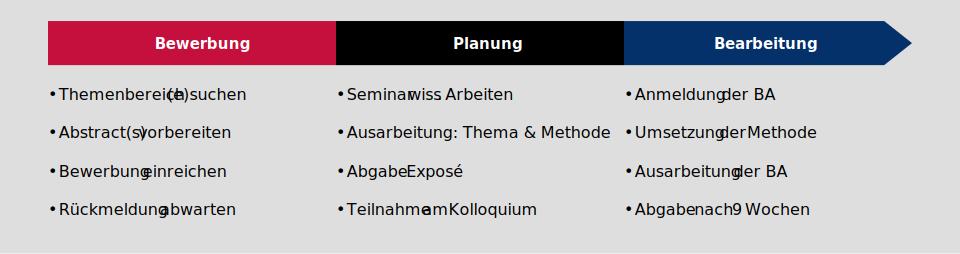
\includegraphics{./img/ablauf.png}

}

\caption{\label{fig-ablauf}Ablauf einer Bachelorarbeit an Lehrstuhl und
Juniorprofessur für Kommunikationswissenschaft}

\end{figure}

\hypertarget{deadlines-bewerbung-vergabe-der-themen}{%
\section{Deadlines, Bewerbung, Vergabe der
Themen}\label{deadlines-bewerbung-vergabe-der-themen}}

Aktuelle Informationen zur Bewerbung, Themenvergabe, Anmeldung und
Abgabe entnehmen Sie bitte der Website des
\href{https://www.kowi.rw.fau.de/studium/abschlussarbeiten/}{Lehrstuhls
für Kommunikationswissenschaft}. In Abbildung~\ref{fig-ablauf} finden
Sie einen Überblick über den Ablauf.

Für Masterarbeiten wenden Sie sich bitte direkt an die Mitarbeiter*innen
des Lehrstuhls und der Juniorprofessur.

\hypertarget{exposuxe9}{%
\section{Exposé}\label{exposuxe9}}

Bitte beachten Sie den Zeitplan auf unserer Website für die
\textbf{Deadline zur Abgabe des Exposés}

Nach den ersten Vorbesprechungen werden Sie gebeten, eine ausführlichere
Projektskizze zum gemeinsam vereinbarten Thema zu erstellen und an Ihre
Betreuungsperson zu senden. Ziel des Exposees ist es sicherzustellen,
dass ein gemeinsames Verständnis von Umfang, Thema und Zielsetzung der
Arbeit entsteht. Das Exposee ist die Grundlage Ihrer Arbeit und
skizziert die weitere Ausarbeitung vor.

Im Exposee erläutern Sie kurz in schriftlicher Form, in welchem
Problemzusammenhang das Thema steht, welche Aspekte und Unteraspekte das
Thema hat, welche Forschungsperspektive Sie einnehmen möchten und welche
Methode(n) zur Beantwortung der Forschungsfrage verwendet werden soll.
Das Dokument sollte insgesamt \textbf{2-4 Seiten} Text (A4, gleiche
Formatierung wie die Abschlussarbeit) umfassen und Folgendes beinhalten:

\begin{itemize}
\item
  Name, Matrikelnummer, Studiengang, Fachsemester, Kontaktdaten
\item
  Arbeitstitel (``Working Title'')
\item
  Ausgangslage, Beschreibung des Themenfeldes und Vorschlag einer
  Fragestellung (ca. 200 Wörter)
\item
  Kurzer Forschungsstand (ca. 100 Wörter)
\item
  Begründung für die Wahl des Themas, Relevanz, Erkenntnisinteresse (ca.
  100 Wörter)
\item
  Ziele, Forschungsfragen (Hypothesen)
\item
  Evtl. Methodik
\item
  Grobgliederung (maximal bis Gliederungsebene 2)
\item
  Literaturliste (erste gesammelte Literatur, Basisliteratur)
\item
  Grober Arbeits- und Zeitplan (Projektaktivitäten)
\end{itemize}

\hypertarget{formalia}{%
\chapter{Formalia}\label{formalia}}

\hypertarget{vorurteilsfreie-sprache}{%
\section{Vorurteilsfreie Sprache}\label{vorurteilsfreie-sprache}}

\hypertarget{allgemeine-hinweise-1}{%
\subsection{Allgemeine Hinweise}\label{allgemeine-hinweise-1}}

Wir empfehlen, in wissenschaftlichen Arbeiten vorurteilsfreie,
geschlechtergerechte Sprache zu verwenden. Im Rahmen kommunikations- und
sozialwissenschaftlicher Forschung beschäftigen wir uns mit Menschen mit
einer Vielfalt von (Geschlechts-) Identitäten, daher ist es wichtig,
diese Realität auch in wissenschaftlichen Arbeiten zu reflektieren und
zu respektieren. Dies schließt ein, ist aber nicht beschränkt auf:

\begin{itemize}
\item
  Geschlechtergerechte Sprache, z.B. \emph{Autor*innen} statt Autoren
\item
  Vorurteilsfreie Sprache, z.B. sollten Sie keine Adjektive als Nomen
  für die Beschreibung von Personen(-gruppen) nutzen
\item
  Hierarchisieren Sie keine Unterschiede zwischen Menschen, z.B. indem
  Sie gesellschaftlich dominante Gruppen in einem Graph über anderen
  Gruppen darstellen
\item
  Quelle und weitere hilfreiche Informationen:
  \href{https://apastyle.apa.org/style-grammar-guidelines/bias-free-language/general-principles}{APA-Styleguide
  zu vorurteilsfreier Sprache}
\end{itemize}

\hypertarget{hinweise-zur-geschlechtergerechten-sprache}{%
\subsection{Hinweise zur geschlechtergerechten
Sprache}\label{hinweise-zur-geschlechtergerechten-sprache}}

Wir empfehlen neutrale Formulierungen oder Formen, die alle
Geschlechtsidentitäten einschließen, z.B. Schüler*innen, Studierende

\begin{itemize}
\item
  Sie können neutrale Formen mit „\emph{:}'' oder „\emph{*}''\footnote{Sie
    müssen dabei keine Rücksicht auf grammatische Konformität nehmen.}
  und/oder Partizipien (\emph{‑ierende}) bilden
\item
  Sie können neutrale Begriffe nutzen, z.B. Person, Beschäftigte
\item
  In englischen Texten können Sie „\emph{they}'' im Singular nutzen
\end{itemize}

Das Verwenden des zwar grammatikalisch korrekten, aber nicht inklusiven
generischen Maskulinums fließt nicht negativ in die Bewertung ein, wir
raten aber dennoch davon ab (s. o.).

\hypertarget{deckblatt-und-verzeichnisse}{%
\section{Deckblatt und
Verzeichnisse}\label{deckblatt-und-verzeichnisse}}

Ihre wissenschaftliche Arbeit sollte ein Deckblatt haben (für ein
Beispiel s. Abbildung~\ref{fig-vorlage_deckblatt})

\begin{figure}

{\centering 
\includegraphics[width=0.66\textwidth,height=\textheight]{./img/vorlage_deckblatt.png}

}

\caption{\label{fig-vorlage_deckblatt}Beispieldeckblatt \textbar{}
{\href{templates/title_page_template.dotx}{Beispielvorlage als
.dotx-Datei herunterladen}}}

\end{figure}

Das Deckblatt sollte folgende Informationen enthalten

\begin{itemize}
\item
  Name der Universität, des Fachbereichs und des Lehrstuhls/der
  Juniorprofessur
\item
  Optional: Logo oder Siegel der Universität
\item
  Modulbezeichnung
\item
  Art der Arbeit (und Seminartitel bei Seminararbeiten)
\item
  Betreuer*in oder Dozent*in des Seminars
\item
  Titel der Arbeit
\item
  Name, Vorname
\item
  Studiengang mit Schwerpunkt
\item
  Zahl der Studiensemester und Fachsemester
\item
  Anschrift mit Telefonnummer
\item
  E-Mail-Adresse
\end{itemize}

Sie benötigen außerdem:

\begin{enumerate}
\def\labelenumi{\arabic{enumi}.}
\tightlist
\item
  ein nummeriertes \textbf{Inhaltsverzeichnis} mit Seitenzahlen, sowie
\item
  \textbf{Abbildungs-}, und/oder
\item
  \textbf{Tabellenverzeichnisse}, wenn Sie Abbildungen und/oder Tabellen
  in Ihrer Arbeit verwenden. Textverarbeitungsprogramme wie Microsoft
  Word können diese automatisch erstellen.
\end{enumerate}

Ein Abkürzungsverzeichnis ist nicht notwendig. Führen Sie stattdessen
zentrale Abkürzungen im Text ein und verzichten Sie ansonsten auf nicht
geläufige Abkürzungen.

\hypertarget{eidesstattliche-erkluxe4rung}{%
\section{Eidesstattliche Erklärung}\label{eidesstattliche-erkluxe4rung}}

Alle wissenschaftlichen Arbeiten, die Sie als Prüfungsleistungen
einreichen, müssen eine Eidesstattliche Erklärung enthalten:

\begin{figure}

\textbf{Eidesstattliche Erklärung}

\{Ich versichere/Wir versichern\}, dass \{ich/wir\} die Arbeit:
``\{Thema\}'' ohne fremde Hilfe und ohne Benutzung anderer als der
angegebenen Quellen angefertigt \{habe(n)\} und dass die Arbeit in
gleicher oder ähnlicher Form noch an keiner anderen Prüfungsbehörde
vorgelegen hat. Alle Ausführungen, die wörtlich übernommen wurden, sind
als solche gekennzeichnet.

\{Unterschrift\}

Ort, Datum \{vollständiger Name\}

\caption{\label{fig-eid}Eidesstattliche Erklärung}

\end{figure}

Hinweise: \{Platzhalter\} in Abbildung~\ref{fig-eid} durch entsprechende
Inhalte ersetzen. Bei Gruppenarbeiten müssen alle Beteiligten eine
eigene Eidesstattliche Erklärung unterschreiben.

\hypertarget{inhalte-einer-wissenschaftlichen-arbeit}{%
\chapter{Inhalte einer wissenschaftlichen
Arbeit}\label{inhalte-einer-wissenschaftlichen-arbeit}}

Wissenschaftliche Arbeiten können diverse Formate einnehmen. Die
Struktur ist vom Gegenstand abhängig, häufig wird aber eine Struktur wie
im Folgenden verwendet.

\hypertarget{gliederung}{%
\section{Gliederung}\label{gliederung}}

\hypertarget{typische-gliederung}{%
\subsection{Typische Gliederung}\label{typische-gliederung}}

Insbesondere bei empirischen Arbeiten oder Literaturüberblicken wird die
folgende typische Struktur verwendet. Abhängig von Inhalt und Art der
Arbeit, ist es nötig, von diesem Schema abzuweichen.

Ihre Gliederung sollte maximal drei Ebenen beinhalten. Kennzeichnen Sie
diese numerisch, z. B. 1., 1.3, 1.4.2, etc. Für eine genauere
Unterscheidung können Sie auf vierter Ebene eine Überschrift zu Beginn
eines Absatzes (eingerückt) einbauen, indem Sie die Überschrift fett
setzen und mit einem Punkt abschließen, z. B.:

\hypertarget{wohlbefinden}{%
\subsubsection{Wohlbefinden}\label{wohlbefinden}}

Wohlbefinden wird definiert als\ldots{} {[}Rest des Absatzes{]}

\hypertarget{beispielgliederung}{%
\subsection{Beispielgliederung}\label{beispielgliederung}}

Beispielgliederung auf erster Ebene einer empirischen Arbeit:

\begin{itemize}
\item
  Abstract (nur bei Abschlussarbeiten; erscheint nicht im
  Inhaltsverzeichnis)
\item
  Inhaltsverzeichnis (nur bei Abschlussarbeiten; erscheint nicht im
  Inhaltsverzeichnis)
\end{itemize}

\begin{enumerate}
\def\labelenumi{\arabic{enumi}.}
\item
  Einleitung
\item
  Theorie und Forschungsstand
\item
  Methodik
\item
  Ergebnisse
\item
  Diskussion
\item
  Literaturverzeichnis
\item
  Anhang, inkl. Tabellen- und Abbildungsverzeichnissen
\end{enumerate}

Im Folgenden wird auf die einzelnen Abschnitte der Arbeit eingegangen.
Alle Abschnitte sollten sinnvoll ineinandergreifen (roter Faden).

\hypertarget{abstract}{%
\section{Abstract}\label{abstract}}

Ein Abstract ist \textbf{nur für Abschlussarbeiten} notwendig, nicht für
Seminararbeiten. Im Abstract werden kurz und knapp alle zentralen
Inhalte der gesamten Arbeit dargestellt. Das Abstract ist für
Leser*innen ein zentrales Entscheidungskriterium für die Relevanz der
Arbeit. Ein wissenschaftliches Abstract sollte kurz, aber vollständig
sein und die wichtigsten Aspekte der Arbeit (Fragestellung, Relevanz,
Forschungslücke, Methode/Design, zentrale Ergebnisse, Implikationen) von
Anfang bis Ende skizziert werden.

\textbf{Anforderungen}: Das Abstract sollte \textbf{150-300 Wörter} lang
sein. Bei Abschlussarbeiten auf Deutsch ist zusätzlich zum deutschen
Abstract ein \textbf{englisches Abstract notwendig}.

\hypertarget{einleitung}{%
\section{Einleitung}\label{einleitung}}

Zu Beginn einer wissenschaftlichen Arbeit sollte der
Untersuchungsgegenstand dargestellt werden. Die Einleitung hat v.a. drei
Ziele:

\begin{enumerate}
\def\labelenumi{\arabic{enumi}.}
\item
  Die \textbf{Relevanz} des Themas herausarbeiten (wissenschaftlich,
  gesellschaftlich, \ldots)
\item
  Einen Aus- und \textbf{Überblick} über die Arbeit bieten
\item
  Das \textbf{Ziel} der Untersuchung darstellen
\end{enumerate}

In vielen Fällen ist es ratsam, in der Einleitung implizit oder explizit
eine \textbf{forschungsleitende Frage} aufzustellen. Diese hilft, den
roten Faden durch die gesamte Arbeit herauszuarbeiten. Anhand der
forschungsleitenden Frage können Sie prüfen, ob nachfolgende Inhalte für
Ihre Arbeit zentral sind (= sie tragen zur Beantwortung der
forschungsleitenden Frage bei) oder weggelassen werden sollten (= sie
tragen nicht zur Beantwortung bei).

Jeder wissenschaftliche Text benötigt eine Einleitung.

\textbf{Umfang}: ca. 5\% des Gesamtumfangs

\hypertarget{hintergrund}{%
\section{Hintergrund}\label{hintergrund}}

Der Hintergrund bildet das theoretische Kernstück der Arbeit. Hier
sollen bisherige Theorien/Konzepte/Modelle sowie der Kenntnisstand
empirischer Forschung zur forschungsleitenden Frage aufgearbeitet
werden.

Dazu sollen Sie zentrale Literatur identifizieren und den theoretischen
Hintergrund herausarbeiten. Bei der Recherche kann es helfen, zunächst
eine zentrale Studie zu suchen, und über dort referenzierte Literatur
weitere Quellen zu finden (sog. ``backward search''). So können auch
ältere, besonders zentrale Beiträge identifiziert werden. Solche Werke
werden wahrscheinlich in gleich mehreren Artikeln referenziert.
Zusätzlich können neuere Studien zum Thema durch einen Blick in die
Beiträge, die eine Schlüsselquelle seit Erscheinen zitiert haben, helfen
(sog. ``forward search'' oder ``citation search'', bspw. über Google
Scholar).

Bei der Recherche stellt sich häufig heraus, dass der Umfang eines
Themengebietes den Rahmen der Arbeit sprengen könnte. In diesen Fällen
sollten Sie Ihr Thema spezifizieren. Der wissenschaftliche Beitrag einer
Arbeit ist größer, wenn ein enges, klar definiertes Thema sehr gut
behandelt wird, als wenn ein breites Thema oberflächlich behandelt wird.
Z. B. könnte die Forschungsfrage „Wie hängt die Smartphone-Nutzung mit
Wohlbefinden zusammen?'' zu „Wie hängen arbeitsbezogene
Smartphone-Benachrichtigungen mit empfundenem Stress zusammen?''
spezifiziert werden. Solche Eingrenzungen des Themas sollten Sie
inhaltlich oder theoretisch begründen können.

\textbf{Umfang}: ca. 20-40\% (kleinerer Anteil bei empirischen, größerer
Anteil bei theoretischen/literaturbasierten Arbeiten)

\hypertarget{methodik}{%
\section{Methodik}\label{methodik}}

Der Methodik-Abschnitt sollte Lesende dazu in die Lage versetzen, Ihre
Arbeit zu reproduzieren. Das beinhaltet beispielsweise die transparente
Darstellung von \textbf{Such-, Einschluss und Ausschlusskriterien} bei
einem Literaturüberblick und die Beschreibung der \textbf{Stichprobe},
verwendeter \textbf{Materialien} und des \textbf{Vorgehen}s bei
empirischen Arbeiten.

Verwendete Materialien, z. B. Fragebögen, Code-Bücher oder
Experimental-Stimuli, gehören in den Anhang.

\textbf{Umfang}: ca. 15-30\%

\hypertarget{ergebnisse}{%
\section{Ergebnisse}\label{ergebnisse}}

Hier werden die Ergebnisse Ihrer Erhebung, Literaturrecherche,
Interviews, etc. dargestellt. Üblicherweise wird hier noch keine
Interpretation der Ergebnisse vorgenommen. Gerade bei
nicht-quantitativen Arbeiten kann in manchen Fällen aber eine stärkere
Integration mit Aspekten der Diskussion oder Theorie sinnvoll sein.

Wichtige Regeln:

\begin{itemize}
\item
  Lateinische Abkürzungen werden kursiv gesetzt und Leerzeichen zwischen
  mathematischen Operatoren eingesetzt (z. B. N=154❌
  vs.~\emph{N}~=~154✅)
\item
  Üblicherweise werden zwei Nachkomastallen angegeben, bei kleinen
  Zahlen (z. B. p-Werten) werden drei Nachkommastellen angegeben:
  \emph{M}~=~15.4383 ❌ \emph{M}~=~15.43 ✅
\item
  Statistiken mit einem Wertebereich von 0 bis 1 werden ohne führende
  Null angegeben: \emph{p} = 0.002 ❌ \emph{p} = .002 ✅
\item
  Verwenden Sie einen Punkt als Dezimaltrennzeichen, Kommas zwischen
  Statistiken und Semikolons, um Sinnabschnitte zu trennen:
  (\emph{t}(123)~=~4.32, \emph{p}~\textless~.001)
\item
  Geben Sie p-Werte immer exakt auf drei Nachkommastellen an, außer der
  Wert ist kleiner als .001, dann geben Sie den Wert mit dem „kleiner
  als'' (\textless) Zeichen an: \emph{p} = .000 ❌
  \emph{p}~\textless~.05 ❌ \emph{p}~\textless~.001 ✅ \emph{p}~=~.045
  ✅
\end{itemize}

In Tabellen und Abbildungen können Sie signifikante Zusammenhänge oder
Effekte durch Sternchen kennzeichnen. Etabliert haben sich * für
\emph{p}~\textless~.05, ** für \emph{p}~\textless~.01 und *** für
\emph{p}~\textless~.001. Eine Erklärung dieser Zeichen gehört in die
Hinweise zur entsprechenden Tabelle/Grafik.

\textbf{Umfang}: ca. 10-20\%

\hypertarget{diskussion}{%
\section{Diskussion}\label{diskussion}}

Hier sollten Sie 1) die Ergebnisse aufgreifen, 2) diese interpretieren
und 3) in den Forschungskontext einordnen. Außerdem werden 4) Stärken
und Schwächen der Arbeit 5) sowie Implikationen für zukünftige
Forschung, die Praxis und/oder die Gesellschaft herausgearbeitet.
Schließlich wird 6) ein Fazit gezogen.

Die Diskussion fügt alle zentralen Teile der Arbeit zusammen und bildet
den Abschluss der Arbeit. Sie beantwortet die in der Einleitung
formulierte übergeordnete Forschungsfrage.

\textbf{Umfang}: ca. 10-20\%

\hypertarget{anhang}{%
\section{Anhang}\label{anhang}}

In den Anhang gehören alle zusätzlichen Informationen, Materialien, etc.
die zur Nachvollziehbarkeit oder zum Verständnis beitragen. Auch
zusätzliche Informationen, wie weitere Analysen, oder Transkripte von
Interviews, etc. gehören hierhin.

\textbf{Umfang}: Der Anhang zählt nicht in den Wortumfang.

\hypertarget{literaturrecherche}{%
\chapter{Literaturrecherche}\label{literaturrecherche}}

Um Fachliteratur zu identifizieren sind spezialisierte Suchmaschinen
hilfreich. Google Scholar listet eine große Menge an aktueller
Fachliteratur sowie grauer Literatur. Fachspezifische Datenbanken,
erreichbar Sie über DBIS der FAU, z. B. PsycInfo oder Scopus, können im
jeweiligen Fachgebiet Literatur anhand von Schlagworten identifizieren.
Für systematischere Suchen können mehrere Begriffe mit logischen
Operatoren (z. B. AND, OR)\footnote{\href{https://libguides.mit.edu/c.php?g=175963\&p=1158594}{Hier
  gibt es mehr Informationen zu logischen Operatoren in Datenbanken}.}
verknüpft werden .

Hilfreiche Links:

\begin{itemize}
\item
  \href{https://ub.fau.de/recherchieren/datenbanken/}{DBIS (Database
  Information System)}

  \begin{itemize}
  \item
    PsycInfo
  \item
    Web of Science
  \item
    Scopus
  \item
    \ldots{}
  \end{itemize}
\item
  \href{https://scholar.google.com/}{Google Scholar}
\item
  \ldots{}
\end{itemize}

Außerdem können Sie\ldots{}

\begin{enumerate}
\def\labelenumi{\arabic{enumi}.}
\tightlist
\item
  \ldots aktuelle Artikel zu Ihrem Thema nutzen, um relevante Beiträge
  zu identifizieren (inkl. ``\emph{forward/citation search}''),
\item
  \ldots die Literaturverzeichnisse von Überblicksartikeln und
  Meta-Analysen nutzen, um relevante Literatur zu identifizieren,
\item
  \ldots zentrale oder bahnbrechende Arbeiten identifizieren und in
  Literatur suchen, die dieser Beitrag zitiert
  (\emph{backward/references search}'').
\end{enumerate}

\hypertarget{open-science}{%
\chapter{Open Science}\label{open-science}}

Im Rahmen von Open Science ermutigen wir Sie, Open-Science Praktiken
umzusetzen, wenn diese angemessen sind, z. B. Ihre Analysen zu
präregistrieren. Eine Präregistrierung schützt vor schlechten
wissenschaftlichen Praktiken, z.B. p-Hacking und HARKing
(``Hypothesizing after results are known'') und kann Ihnen die
Sicherheit geben, dass Ihre Hypothesen und Analysen schon vor dem
Erhebungsbeginn feststehen. Es gibt verschiedene Formen der
Präregistrierung. Bei der einfachsten Form sind
Hypothesen/Forschungsfragen, gemessene und/oder manipulierte Variablen,
Analysen (z. B. Regression, t-test, ANOVA), und geplante
Stichprobengröße enthalten. Sie können
\href{https://aspredicted.org}{aspredicted.org} nutzen, um eine einfache
Präregistrierung in Absprache mit der betreuenden Person Ihrer
Bachelorarbeit zu erstellen.

Für mehr Informationen gibt es die Agenda for Open Science in
Communication (Dienlin et al., 2021)

\hypertarget{zitieren}{%
\chapter{Zitieren}\label{zitieren}}

Wir erwarten, dass Sie alle fremden Gedanken kennzeichnen. In der
Wissenschaft stützen wir uns auf die „Schultern von Riesen'', d.h. Sie
sollten Ihre Arbeit auf bestehender Literatur aufbauen und vorherigen
Leistungen ``Credit geben''. Die vorhandene wissenschaftliche Literatur
zu nutzen, macht Ihre Arbeit theoretisch, inhaltlich und methodisch
stärker.

Sie sollten nach den Richtlinien des Publication Manuals (7. Ausgabe)
der American Psychological Association {[}APA{]} (2020), kurz APA7,
zitieren. Sie finden übersichtliche und anschauliche Anleitungen,
Beispiele, etc. dazu online auf der \href{https://apastyle.apa.org/}{APA
Style-Seite} (o.~J.).

\textbf{Achtung}: \emph{Abweichend von den APA-Richtlinien verlangen
wir, dass Sie in Kurzbelegen Seitenanzahlen angeben} (s.
Abschnitt~\ref{sec-indirect}). Ausgenommen hiervon sind Verweise auf
einen gesamten Beitrag oder das ungefähre Thema.

Wir empfehlen, dass Sie ein Zitationsprogramm wie
\href{https://www.zotero.org/}{Zotero} (kostenlos, open source), Citavi
oder Endnote nutzen. Bedenken Sie, dass diese Programme nur korrekt
arbeiten, wenn Sie die richtigen Informationen in die vorgesehenen
Felder eingeben und den APA7 Zitationsstil auswählen.

Sprache: In Deutschen Arbeiten dürfen Sie grundsätzlich auf Deutsch oder
Englisch zitieren, z. B. Hrsg. vs.~Eds., oder S. 4 vs.~p.~4. Wir
empfehlen die englische APA7-Schreibweise aufgrund der weiter
verbreiteten Integration in Zitationsprogramme. In englischen Arbeiten
sollten Sie englisch zitieren. Titel, Publikationsnamen, etc. werden
nicht übersetzt.

Im Folgenden finden Sie eine Kurzanleitung\footnote{Die Anleitung zum
  Zitieren basiert auf einem Kurz-Manual das vom
  \href{https://www.medienpsychologie.ifp.uni-mainz.de/}{Lehrstuhl
  Medienwirkung \& Medienpsychologie} an der JGU Mainz
  (Prof.~Dr.~Leonard Reinecke) erstellt wurde. Besonderer Dank gebührt
  Alicia Ernst, Alicia Gilbert und Anisha Arenz.}. \textbf{Wichtig}: Sie
können diesen Abschnitt als Nachschlagewerk nutzen, müssen ihn aber
nicht vollständig durcharbeiten.

\hypertarget{die-huxe4ufigsten-literaturangaben}{%
\section{Die häufigsten
Literaturangaben}\label{die-huxe4ufigsten-literaturangaben}}

Der Großteil Ihrer Quellen wird in der Regel aus den folgenden
Literaturtypen bestehen:

\hypertarget{monographie}{%
\subsection{Monographie:}\label{monographie}}

Koch, T. (2010). \emph{Macht der Gewohnheit? Der Einfluss der
Habitualisierung auf die Fernsehnutzung}. VS Verlag für
Sozialwissenschaften. \url{https://doi.org/10.1007/978-3-531-92529-5}

\hypertarget{zeitschriftenaufsatz}{%
\subsection{Zeitschriftenaufsatz}\label{zeitschriftenaufsatz}}

Horton, D., \& Wohl, R. R. (1956). Mass communication and para-social
interaction: Observations on intimacy at a distance. \emph{Psychiatry,
19}(3), 215--229.
\href{https://doi.org/10.1080/00-\%20332747.1956.11023049}{https://doi.org/10.1080/00-
332747.1956.11023049}

\hypertarget{beitrag-in-einem-sammelband}{%
\subsection{Beitrag in einem
Sammelband}\label{beitrag-in-einem-sammelband}}

Huta, V. (2017). An overview of hedonic and eudaimonic well-being
concepts. In L. Reinecke \& M. B. Oliver (Eds.), \emph{The Routledge
handbook of media use and well-being. International perspectives on
theory and research on positive media effects} (pp.~14--33). Routledge.

\hypertarget{beitrag-auf-einer-nachrichtenwebsite}{%
\subsection{Beitrag auf einer
Nachrichtenwebsite}\label{beitrag-auf-einer-nachrichtenwebsite}}

Roller-Spoo, J. (2020, October 24). \emph{Von Hatern und Hetzern: Der
Kampf gegen Hass im Netz}. ZDF heute--Nachrichten.
https://www.zdf.de/nachrichten/digitales/hate-speech-hass-gewalt-internet-100.html

\hypertarget{sec-angaben-im-literaturverzeichnis}{%
\section{Angaben im
Literaturverzeichnis}\label{sec-angaben-im-literaturverzeichnis}}

\hypertarget{sec-buxfccher-und-ebooks}{%
\subsection{Bücher und eBooks}\label{sec-buxfccher-und-ebooks}}

\hypertarget{tbl-monographs}{}
\begin{longtable}[]{@{}
  >{\raggedright\arraybackslash}p{(\columnwidth - 8\tabcolsep) * \real{0.2155}}
  >{\raggedright\arraybackslash}p{(\columnwidth - 8\tabcolsep) * \real{0.0718}}
  >{\raggedright\arraybackslash}p{(\columnwidth - 8\tabcolsep) * \real{0.2707}}
  >{\raggedright\arraybackslash}p{(\columnwidth - 8\tabcolsep) * \real{0.2928}}
  >{\raggedright\arraybackslash}p{(\columnwidth - 8\tabcolsep) * \real{0.1326}}@{}}
\caption{\label{tbl-monographs}Allgemeines Zitationsschema für
Monographien und Sammelbände}\tabularnewline
\toprule()
\begin{minipage}[b]{\linewidth}\raggedright
Autor*in
\end{minipage} & \begin{minipage}[b]{\linewidth}\raggedright
Jahr
\end{minipage} & \begin{minipage}[b]{\linewidth}\raggedright
Titel
\end{minipage} & \begin{minipage}[b]{\linewidth}\raggedright
Quelle: Verlag
\end{minipage} & \begin{minipage}[b]{\linewidth}\raggedright
Quelle: doi/URL
\end{minipage} \\
\midrule()
\endfirsthead
\toprule()
\begin{minipage}[b]{\linewidth}\raggedright
Autor*in
\end{minipage} & \begin{minipage}[b]{\linewidth}\raggedright
Jahr
\end{minipage} & \begin{minipage}[b]{\linewidth}\raggedright
Titel
\end{minipage} & \begin{minipage}[b]{\linewidth}\raggedright
Quelle: Verlag
\end{minipage} & \begin{minipage}[b]{\linewidth}\raggedright
Quelle: doi/URL
\end{minipage} \\
\midrule()
\endhead
Autor*in, A. A., \& Autor*in, B. B.

Name einer Gruppe/Organisation

Herausgeber*in, E. E. (Ed.).

Herausgeber*in, E. E., \&

Herausgeber*in, F. F. (Eds.). & (2020) & \emph{Name des Buchs.}

\emph{Name des Buchs} (2nd Ed., Vol. 4).

\emph{Name des Buchs} (E. E. Herausgeber*in, Ed.).

\emph{Name des Buchs} (Ü. Übersetzer*in, Trans.). & Verlagsname.

Name des ersten Verlags; Name des zweiten Verlags. &
\url{https://doi.org.xxx}

\url{https://xxx} \\
\bottomrule()
\end{longtable}

\hypertarget{allgemeine-hinweise-2}{%
\subsubsection{\texorpdfstring{\textbf{Allgemeine
Hinweise}}{Allgemeine Hinweise}}\label{allgemeine-hinweise-2}}

\begin{itemize}
\item
  Nennen Sie Autor*in, Erscheinungsjahr, Titel sowie den Namen des
  Verlags.
\item
  Nennen Sie jegliche Informationen über eine neue Auflage in einer
  Klammer nach dem Titel ohne Kursivsetzung.
\item
  Wenn das Buch einen Digital Object Identifier (doi) hat, nennen Sie
  die doi-Nummer als Link nach dem Namen des Verlags, bspw.
  \url{https://doi.org/10.1234/j.soscij.2020.-12.34}. Andere
  Nummernsysteme (z.B. ISBN) werden im APA-Stil nicht verwendet.
\item
  Nennen Sie keinen Verlagsort.
\item
  Wenn das Buch keine doi besitzt und ein eBook einer wissenschaftlichen
  Datenbank ist, endet die Literaturangabe nach dem Verlagsnamen. Nennen
  Sie keine Datenban-kinformationen. Die Literaturangabe gleicht dann
  der von Printausgaben.
\item
  Wenn ein Buch 20 Autor*innen oder weniger besitzt, nennen Sie alle
  Autor*innen. Wenn ein Buch 21 Autor*innen oder mehr besitzt, nennen
  Sie die ersten 19 Autor*innen, setzen Sie danach drei Punkte
  („\ldots``) und nennen Sie danach den Namen der/des letzten Autor*in.
  Diese Regel gilt auch für Zeitschriftenartikel (s.
  Abschnitt~\ref{sec-fachzeitschriften}).
\end{itemize}

\hypertarget{monographien}{%
\subsection{Monographien}\label{monographien}}

\hypertarget{monographie-eine-autorin-mit-doi}{%
\subsubsection{Monographie \textbar{} ein*e Autor*in \textbar{} mit
doi}\label{monographie-eine-autorin-mit-doi}}

Koch, T. (2010). \emph{Macht der Gewohnheit? Der Einfluss der
Habitualisierung auf die Fernsehnutzung}. VS Verlag für
Sozialwissenschaften. \url{https://doi.org/10.1007/978-3-531-92529-5}

\hypertarget{monographie-eine-autorin-ohne-doi}{%
\subsubsection{Monographie \textbar{} ein*e Autor*in \textbar{} ohne
doi}\label{monographie-eine-autorin-ohne-doi}}

Donsbach, W. (1982). \emph{Legitimationsprobleme des Journalismus:
Gesellschaftliche Rolle der Massenmedien und berufliche Einstellungen
von Journalisten}. Alber-Verlag.

\hypertarget{monographie-zwei-bis-21-autorinnen-ohne-doi}{%
\subsubsection{Monographie \textbar{} zwei bis 21 Autor*innen \textbar{}
ohne doi}\label{monographie-zwei-bis-21-autorinnen-ohne-doi}}

Lazarsfeld, P. F., Berelson, B., \& Gaudet, H. (1968). \emph{The
people's choice: How the voter makes up his mind in a presidential
campaign}. Columbia University Press.

\hypertarget{monographie-uxfcbersetzung-ohne-doi}{%
\subsubsection{Monographie \textbar{} Übersetzung \textbar{} ohne
doi}\label{monographie-uxfcbersetzung-ohne-doi}}

Freud, S. (1970). \emph{An outline of psychoanalysis} (J. Strachey,
Trans.). Norton. (Original work published 1940)

\hypertarget{monographie-band-in-einer-reihe-mit-doi}{%
\subsubsection{Monographie \textbar{} Band in einer Reihe \textbar{} mit
doi}\label{monographie-band-in-einer-reihe-mit-doi}}

Kepplinger, H. M. (2011). \emph{Journalismus als Beruf}. VS Verlag für
Sozialwissenschaften. \url{https://doi.org/10.1007/978-3-531-92915-6}

\emph{Anmerkung}: bei einem Band in einer Reihe, in der einzelne Bände
nur konzeptuell verwandt sind, wird der Titel der Reihe nicht genannt.
Der Titel der Schriftenreihe wäre hier Theorie und Praxis öffentlicher
Kommunikation.

\hypertarget{sammelbuxe4nde}{%
\subsection{Sammelbände}\label{sammelbuxe4nde}}

\hypertarget{sammelband-zwei-bis-21-herausgeberinnen-ohne-doi}{%
\subsubsection{Sammelband \textbar{} zwei bis 21 Herausgeber*innen
\textbar{} ohne
doi}\label{sammelband-zwei-bis-21-herausgeberinnen-ohne-doi}}

Reinecke, L., \& Oliver, M. B. (Eds.). (2016). \emph{The Routledge
handbook of media use and well-being}. Routledge.

\hypertarget{sammelband-mit-mehreren-buxe4nden-band-ohne-eigenen-titel-neue-auflage-mit-doi}{%
\subsubsection{Sammelband mit mehreren Bänden \textbar{} Band ohne
eigenen Titel \textbar{} neue Auflage \textbar{} mit
doi}\label{sammelband-mit-mehreren-buxe4nden-band-ohne-eigenen-titel-neue-auflage-mit-doi}}

Fiske, S. T., Gilbert, D. T., \& Lindzey, G. (Eds.). (2010). Handbook of
social psychology (5th Ed., Vol. 1). John Wiley \& Sons.
\url{https://doi.org/10.1002/9780470561119}

\hypertarget{sammelband-mit-mehreren-buxe4nden-band-mit-eigenem-titel-mit-doi}{%
\subsubsection{Sammelband mit mehreren Bänden \textbar{} Band mit
eigenem Titel \textbar{} mit
doi}\label{sammelband-mit-mehreren-buxe4nden-band-mit-eigenem-titel-mit-doi}}

Travis, C. B., \& White, J. W. (Eds.). (2018). \emph{APA handbook of the
psychology of women}: Vol. 1. History, theory, and battlegrounds.
American Psychological Association.
\url{https://doi.org/10.1037/0000059-000}

\hypertarget{sammelband-in-einer-reihe-mit-doi}{%
\subsubsection{Sammelband in einer Reihe \textbar{} mit
doi}\label{sammelband-in-einer-reihe-mit-doi}}

Pollock, G., Ozan, J., Goswami, H., Rees, G., \& Stasulane, A. (Eds.).
(2018). \emph{Measuring youth well-being: How a pan-European
longitudinal survey can improve policy}. Springer International
Publishing. \url{https://doi.org/10.1007/978-3-319-76063-6}

\emph{Anmerkung}: bei einem Band in einer Reihe, in der einzelne Titel
nur konzeptuell verwandt sind, wird der Titel der Reihe nicht genannt.
Der Titel der Schriftenreihe wäre hier Children's well-being: Indicators
and research.

\hypertarget{tagungsband-wird-zitiert-wie-ein-sammelband-ohne-doi}{%
\subsubsection{Tagungsband (wird zitiert wie ein Sammelband) \textbar{}
ohne doi}\label{tagungsband-wird-zitiert-wie-ein-sammelband-ohne-doi}}

Kalch, A., \& Wagner, A. (Eds.). (2020). \emph{Gesundheitskommunikation
und Digitalisierung: Zwischen Lifestyle, Prävention und
Krankheitsversorgung}. Nomos.

\hypertarget{kapitel-oder-beitrag-in-einem-sammelband-ohne-doi}{%
\subsubsection{Kapitel oder Beitrag in einem Sammelband \textbar{} ohne
doi}\label{kapitel-oder-beitrag-in-einem-sammelband-ohne-doi}}

Huta, V. (2017). An overview of hedonic and eudaimonic well-being
concepts. In L. Reinecke \& M. B. Oliver (Eds.), \emph{The Routledge
handbook of media use and well-being. International perspectives on
theory and research on positive media effects} (pp.~14--33). Routledge.

\hypertarget{beitrag-in-einem-sammelband-mit-mehreren-buxe4nden-mit-doi}{%
\subsubsection{Beitrag in einem Sammelband mit mehreren Bänden
\textbar{} mit
doi}\label{beitrag-in-einem-sammelband-mit-mehreren-buxe4nden-mit-doi}}

Roberts, T.-A., Calogero, R. M., \& Gervais, S. J. (2018).
Objectification theory: Continuing contributions to feminist psychology.
In C. B. Travis \& J. W. White (Eds.), APA handbook of the psychology of
women: Vol. 1. History, theory, and battlegrounds. American
Psychological Association. \url{https://doi.org/10.1037/0000059-000}

\hypertarget{beitrag-in-einer-enzyklopuxe4die-mit-doi}{%
\subsubsection{Beitrag in einer Enzyklopädie \textbar{} mit
doi}\label{beitrag-in-einer-enzyklopuxe4die-mit-doi}}

Valkenburg, P. M., \& Peter, J. (2017). Differential susceptibility to
media effects model. In P. Rössler, C. A. Hoffner, \& L. Zoonen (Eds.),
The international encyclopedia of media effects. John Wiley \& Sons.
\url{https://doi.org/10.1002/9781118783764.wbieme0119}

\hypertarget{sec-fachzeitschriften}{%
\subsection{Fachzeitschriften}\label{sec-fachzeitschriften}}

\hypertarget{tbl-journal}{}
\begin{longtable}[]{@{}
  >{\raggedright\arraybackslash}p{(\columnwidth - 8\tabcolsep) * \real{0.2516}}
  >{\raggedright\arraybackslash}p{(\columnwidth - 8\tabcolsep) * \real{0.1321}}
  >{\raggedright\arraybackslash}p{(\columnwidth - 8\tabcolsep) * \real{0.1384}}
  >{\raggedright\arraybackslash}p{(\columnwidth - 8\tabcolsep) * \real{0.3082}}
  >{\raggedright\arraybackslash}p{(\columnwidth - 8\tabcolsep) * \real{0.1509}}@{}}
\caption{\label{tbl-journal}Schema für Fachzeitschriften}\tabularnewline
\toprule()
\begin{minipage}[b]{\linewidth}\raggedright
Autor*in
\end{minipage} & \begin{minipage}[b]{\linewidth}\raggedright
Jahr
\end{minipage} & \begin{minipage}[b]{\linewidth}\raggedright
Titel
\end{minipage} & \begin{minipage}[b]{\linewidth}\raggedright
Quelle: Verlag
\end{minipage} & \begin{minipage}[b]{\linewidth}\raggedright
Quelle: doi/URL
\end{minipage} \\
\midrule()
\endfirsthead
\toprule()
\begin{minipage}[b]{\linewidth}\raggedright
Autor*in
\end{minipage} & \begin{minipage}[b]{\linewidth}\raggedright
Jahr
\end{minipage} & \begin{minipage}[b]{\linewidth}\raggedright
Titel
\end{minipage} & \begin{minipage}[b]{\linewidth}\raggedright
Quelle: Verlag
\end{minipage} & \begin{minipage}[b]{\linewidth}\raggedright
Quelle: doi/URL
\end{minipage} \\
\midrule()
\endhead
Autor*in, A. A., \& Au-tor*in, B. B.

Name einer Gruppe/Organisation & (2020).

(2020, January).

(2020, January 1). & Titel des Artikels. & \emph{Titel der Zeitschrift,
34}(2), 5--14.

\emph{Titel der Zeitschrift, 15}(1--2), Article 12.

\emph{Titel der Zeitschrift}. & \url{https://doi.org.xxx}

\url{https://xxx} \\
\bottomrule()
\end{longtable}

\hypertarget{allgemeine-hinweise-3}{%
\subsubsection{\texorpdfstring{\textbf{Allgemeine
Hinweise}}{Allgemeine Hinweise}}\label{allgemeine-hinweise-3}}

\begin{itemize}
\item
  Wenn ein Aufsatz eine doi-Nummer hat, geben Sie die doi an.
\item
  Geben Sie bei Zeitschriftenaufsätzen, wenn vorhanden, immer die
  Heftnummer an.
\item
  Wenn ein Zeitschriftenaufsatz keine doi besitzt und von einer
  wissenschaftlichen Datenbank stammt, beenden Sie die Angabe mit der
  Angabe der Seitenspanne.
\item
  Wenn der Zeitschriftenaufsatz keine doi besitzt, aber dafür eine URL,
  nennen Sie stattdessen die URL am Ende der Literaturangabe.
\item
  Wenn der Zeitschriftenaufsatz eine Artikelnummer (z.B. e12345678)
  anstelle einer Sei-tenangabe hat, nennen Sie das Wort „Artikel'' und
  folgend die Artikelnummer.
\item
  Wenn ein Zeitschriftenartikel 20 Autor*innen oder weniger besitzt,
  nennen Sie alle Autor*innen. Wenn ein Artikel 21 Autor*innen oder mehr
  besitzt, nennen Sie die ersten 19 Autor*innen, setzen Sie danach drei
  Punkte („\ldots``) und nennen Sie danach den Namen der/des letzten
  Autor*in. Diese Regel gilt auch für Bücher (s.
  Abschnitt~\ref{sec-bücher-und-ebooks}).
\end{itemize}

\hypertarget{publizierte-zeitschriftenaufsuxe4tze-in-wissenschaftlichen-fachzeitschriften.}{%
\subsection{Publizierte Zeitschriftenaufsätze in wissenschaftlichen
Fachzeitschriften.}\label{publizierte-zeitschriftenaufsuxe4tze-in-wissenschaftlichen-fachzeitschriften.}}

\hypertarget{zeitschriftenaufsatz-eine-autorin-mit-doi}{%
\subsubsection{Zeitschriftenaufsatz \textbar{} ein*e Autor*in \textbar{}
mit doi}\label{zeitschriftenaufsatz-eine-autorin-mit-doi}}

Walther, J. B. (1996). Computer-mediated communication: Impersonal,
interpersonal, and hyperpersonal interaction. \emph{Communication
Research, 23}(1), 3--43.
\url{https://doi.org/10.1177/009365096023001001}

\hypertarget{zeitschriftenaufsatz-zwei-bis-21-autorinnen-ohne-heftnummer-mit-doi}{%
\subsubsection{Zeitschriftenaufsatz \textbar{} zwei bis 21 Autor*innen
\textbar{} ohne Heftnummer \textbar{} mit
doi}\label{zeitschriftenaufsatz-zwei-bis-21-autorinnen-ohne-heftnummer-mit-doi}}

Appel, H., Gerlach, A. L., \& Crusius, J. (2016). The interplay between
Facebook use, social comparison, envy, and depression. \emph{Current
Opinion in Psychology, 9}, 44--49.
\url{https://doi.org/10.1016/j.copsyc.2015.10.006}

\hypertarget{zeitschriftenaufsatz-zwei-bis-21-autorinnen-mit-heftnummer-mit-doi}{%
\subsubsection{Zeitschriftenaufsatz \textbar{} zwei bis 21 Autor*innen
\textbar{} mit Heftnummer \textbar{} mit
doi}\label{zeitschriftenaufsatz-zwei-bis-21-autorinnen-mit-heftnummer-mit-doi}}

Horton, D., \& Wohl, R. R. (1956). Mass communication and para-social
interaction: Observations on intimacy at a distance. \emph{Psychiatry,
19}(3), 215--229. \url{https://doi.org/10.1080/00332747.1956.11023049}

\hypertarget{zeitschriftenaufsatz-zwei-bis-21-autorinnen-mit-artikel-id-mit-doi}{%
\subsubsection{Zeitschriftenaufsatz \textbar{} zwei bis 21 Autor*innen
\textbar{} mit Artikel ID \textbar{} mit
doi}\label{zeitschriftenaufsatz-zwei-bis-21-autorinnen-mit-artikel-id-mit-doi}}

Reinecke, L., Klimmt, C., Meier, A., Reich, S., Hefner, D., Knop-Huelss,
K., Rieger, D., \&, Vorderer, P. (2018). Permanently online and
permanently connected: Development and validation of the Online
Vigilance Scale. \emph{PLoS ONE, 13}(10), Article e0205384.
\url{https://doi.org/10.1371/journal.pone.0205384}

\hypertarget{zeitschriftenaufsatz-21-oder-mehr-autorinnen-autorinnenregel-gilt-auch-fuxfcr-buxfccher-mit-heftnummer-mit-doi}{%
\subsubsection{Zeitschriftenaufsatz \textbar{} 21 oder mehr Autor*innen
(Autor*innenregel gilt auch für Bücher) \textbar{} mit Heftnummer
\textbar{} mit
doi}\label{zeitschriftenaufsatz-21-oder-mehr-autorinnen-autorinnenregel-gilt-auch-fuxfcr-buxfccher-mit-heftnummer-mit-doi}}

Rumpf, H.-J., Achab, S., Billieux, J., Bowden-Jones, H., Carragher, N.,
Demetrovics, Z., Hi-guchi, S., King, D. L., Mann, K., Potenza, M.,
Saunders, J. B., Abbott, M., Ambekar, A., Aricak, O. T.,
Assanangkornchai, S., Bahar, N., Borges, G., Brand, M., Chan, E. M.-L.,
. . . Poznyak, V. (2018). Including gaming disorder in the ICD-11: The
need to do so from a clinical and public health perspective.
\emph{Journal of Behavioral Addictions, 7}(3), 556--561.
\url{https://doi.org/10.1556/2006.7.2018.59}

\hypertarget{vorabpublikationen-wissenschaftlicher-fachzeitschriftenartikel-preprints}{%
\subsection{Vorabpublikationen wissenschaftlicher
Fachzeitschriftenartikel
(``Preprints'')}\label{vorabpublikationen-wissenschaftlicher-fachzeitschriftenartikel-preprints}}

Bei einer Recherche im Internet können Sie manchmal auf Vorabversionen
von Fachzeitschriftenartikeln stoßen (sog. „Preprints''). Da diese
Vorabversionen oft von der publizierten Version abweichen, sollten Sie
eine Vorabpublikation als solche kennzeichnen: Zitieren Sie also die
Vorabversion eines Werkes gemäß den unten genannten Beispielen, falls
Sie diese in Ihrer Arbeit verwenden. Dies gilt nicht nur für
Zeitschriftenaufsätze, sondern auch für Sammelbände und Monographien.
Idealerweise benutzen und zitieren Sie die finale, publizierte Version
des Werkes, wenn diese vorliegt. Manchmal trifft man bei Quellenangaben
auch auf die Bezeichnung „in press'' oder „im Druck''. Dabei handelt es
sich um Publikationen, die kurz vor der Veröffentlichung stehen, aber
noch nicht öffentlich zugänglich sind.

\hypertarget{zeitschriftenaufsatz-vorabdruck-preprint-aus-einer-datenbank-bspw.-psyarxiv-oder-pubmed-central}{%
\subsubsection{Zeitschriftenaufsatz \textbar{} Vorabdruck („Preprint'')
aus einer Datenbank (bspw. PsyArXiv oder PubMed
Central)}\label{zeitschriftenaufsatz-vorabdruck-preprint-aus-einer-datenbank-bspw.-psyarxiv-oder-pubmed-central}}

Meier, A., \& Reinecke, L. (2020). \emph{Computer-mediated
communication, social media, and mental health: A conceptual and
empirical meta-review}. PsyArXiv.
\url{https://doi.org/10.31234/osf.io/573ph}

\hypertarget{zeitschriftenaufsatz-online-publikation-vorab-verfuxfcgbar-engl.-advance-online-publication}{%
\subsubsection{Zeitschriftenaufsatz \textbar{} Online-Publikation vorab
verfügbar (engl. Advance Online
Publication)}\label{zeitschriftenaufsatz-online-publikation-vorab-verfuxfcgbar-engl.-advance-online-publication}}

Tai, Y., \& Fu, K. (2020). Specificity, conflict, and focal point: A
systematic investigation into social media censorship in China.
\emph{Journal of Communication}. Advance online publication.
\url{https://doi.org/10.1093/joc/jqaa032}

\hypertarget{zeitschriftenaufsatz-im-druck}{%
\subsubsection{Zeitschriftenaufsatz \textbar{} „im
Druck''}\label{zeitschriftenaufsatz-im-druck}}

Turney, P. D. (in press). The latent relation mapping engine: Algorithm
and experiments. \emph{Journal of Artifical Intelligence Research}.

\hypertarget{weitere-wissenschaftliche-beitruxe4ge}{%
\subsection{Weitere wissenschaftliche
Beiträge}\label{weitere-wissenschaftliche-beitruxe4ge}}

\hypertarget{bericht-einer-organisation-oder-institution-als-autorin-url-anstelle-einer-doi}{%
\subsubsection{Bericht einer Organisation oder Institution als Autor*in
\textbar{} URL anstelle einer
doi}\label{bericht-einer-organisation-oder-institution-als-autorin-url-anstelle-einer-doi}}

Pew Research Center. (2020). \emph{Parenting children in the age of
screens}.
\url{https://www.pewresearch.org/internet/2020/07/28/parenting-children-in-the-age-of-screens/}

\hypertarget{bericht-von-autorinnen-innerhalb-einer-organisation-url-anstelle-einer-doi}{%
\subsubsection{Bericht von Autor*innen innerhalb einer Organisation
\textbar{} URL anstelle einer
doi}\label{bericht-von-autorinnen-innerhalb-einer-organisation-url-anstelle-einer-doi}}

Fried, D., \& Polyakova, A. (2018). \emph{Democratic defense against
disinformation}. Atlantic Council.
\url{https://www.atlanticcouncil.org/images/publications/Democratic_Defense_Against_Disinformation_FINAL.pdf}

\hypertarget{pruxe4sentation-eines-beitrags-auf-einer-tagung-ohne-url}{%
\subsubsection{Präsentation eines Beitrags auf einer Tagung \textbar{}
ohne
URL}\label{pruxe4sentation-eines-beitrags-auf-einer-tagung-ohne-url}}

Freytag, A., Knop-Huelss, K., Hefner, D., Klimmt, C., Reinecke, L.,
Meier, A., \& Vorderer, P. (2019, May 24.--28.). \emph{Permanently
online and always stressed out? The effects of online vigilance on
digital stress experiences} {[}Conference contribution{]}. 69th Annual
Conference of the International Communication Association (ICA), Prague,
Czech Republic.

\hypertarget{posterpruxe4sentation-auf-einer-tagung-mit-url}{%
\subsubsection{Posterpräsentation auf einer Tagung \textbar{} mit
URL}\label{posterpruxe4sentation-auf-einer-tagung-mit-url}}

Schneiders, P. (2020, March 10.--12.). \emph{Inhalt erinnert, Quelle
vergessen? Faktoren eines effektiven Social Brandings von
Nachrichtenorganisationen} {[}Poster presentation{]}. 65. Jahrestagung
der Deutschen Gesellschaft für Publizistik- und
Kommunikationswissenschaft (DGPuK), Munich, Germany.
\url{https://www.conftool.org/dgpuk2020/}

\hypertarget{dissertation-von-einer-datenbank-mit-url}{%
\subsubsection{Dissertation von einer Datenbank \textbar{} mit
URL}\label{dissertation-von-einer-datenbank-mit-url}}

Sharp, D. C. (2020). \emph{Waiting to connect: In pursuit of
belongingness and connectedness needs for girls through social network
sites} (Publication No.~27837279) {[}Dissertation, Oklahoma State
University{]}. ProQuest Dissertations and Theses Global.

\hypertarget{online-veruxf6ffentlichung-einer-masterarbeit-von-einer-universituxe4tswebsite-mit-url}{%
\subsubsection{Online Veröffentlichung einer Masterarbeit von einer
Universitätswebsite \textbar{} mit
URL}\label{online-veruxf6ffentlichung-einer-masterarbeit-von-einer-universituxe4tswebsite-mit-url}}

Wilson, B. R. (2018). \emph{Motivating oneself to be physically active
through selective use of so- cial media imagery}. {[}Master's thesis,
The Ohio State University{]}. OhioLINK Electronic Theses and
Dissertations Center.
\url{https://etd.ohiolink.edu/!etd.send_file?accession=osu1530192099884859\&disposition=inline}

\hypertarget{unpublizierte-dissertation}{%
\subsubsection{Unpublizierte
Dissertation}\label{unpublizierte-dissertation}}

Meier, A. (2020). \emph{Do social media make us (un)happy? A
communication-centered approach} {[}Unpublished doctoral
dissertation{]}. Johannes Gutenberg-Universität Mainz.

\hypertarget{online-erguxe4nzungsmaterial-engl.-online-supplement}{%
\subsubsection{Online Ergänzungsmaterial (engl. Online
Supplement)}\label{online-erguxe4nzungsmaterial-engl.-online-supplement}}

Freeberg, T. M. (2019). From simple rules of individual proximity,
complex and coordinated collective movement {[}Supplement{]}.
\emph{Journal of Comparative Psychology, 133}(2), 141--142.
\url{https://doi.org/10.1037/com0000181}

\hypertarget{journalismus-und-onlinemedien}{%
\subsection{Journalismus und
Onlinemedien}\label{journalismus-und-onlinemedien}}

\hypertarget{zeitungsartikel-print}{%
\subsubsection{Zeitungsartikel (Print)}\label{zeitungsartikel-print}}

Menne, K. (2020, October 8.). Superrechner ausgebremst. \emph{DIE ZEIT},
p.~34.

\hypertarget{magazin-print}{%
\subsubsection{Magazin (Print)}\label{magazin-print}}

Ackermann, S. (2020, August). Plötzlich nicht mehr erreichbar.
\emph{Psychologie Heute, 47}(8), 68--72.

\hypertarget{artikel-auf-einer-nachrichtenwebsite}{%
\subsubsection{Artikel auf einer
Nachrichtenwebsite}\label{artikel-auf-einer-nachrichtenwebsite}}

Roller-Spoo, J. (2020, October 24). \emph{Von Hatern und Hetzern‎: Der
Kampf gegen Hass im Netz‎}. ZDF heute--Nachrichten.
\url{https://www.zdf.de/nachrichten/digitales/hate-speech-hass-gewalt-internet-100.html}

Hegemann, L. (2020, October 22). \emph{Wenn der Nachrichtendienst Ihren
WhatsApp-Chat mitlesen will}. ZEIT ONLINE.
\url{https://www.zeit.de/digital/datenschutz/2020-10/ueberwachung-geheimdienste-datensschutz-warnung-staatstrojaner-bundesregierung-schadsoftware}

\hypertarget{beitrag-auf-einer-website-mit-sich-stetig-aktualisierenden-und-nicht-archivierten-informationen}{%
\subsubsection{Beitrag auf einer Website mit sich stetig
aktualisierenden und nicht archivierten
Informationen}\label{beitrag-auf-einer-website-mit-sich-stetig-aktualisierenden-und-nicht-archivierten-informationen}}

U.S. Census Bureau. (n.d.). \emph{U.S. and world population clock}. U.S.
Department of Commerce. Retrieved Juli 3, 2019, from
\url{https://www.census.gov/popclock/}

\hypertarget{beitrag-in-einem-online-wuxf6rterbuch}{%
\subsubsection{Beitrag in einem
Online-Wörterbuch}\label{beitrag-in-einem-online-wuxf6rterbuch}}

Dudenredaktion (n.d.). Medium, das. In \emph{Duden Online}. Retrieved
October 25, 2020, from
\url{https://www.duden.de/rechtschreibung/Medium_Vermittler_Traeger}

\hypertarget{blog-post}{%
\subsubsection{Blog Post}\label{blog-post}}

Rohrer, J. (2019, October 3). Indirect Effect Ex Machina. \emph{The
100\% CI}.
\url{http://www.the100.ci/2019/10/03/indirect-effect-ex-machina/}

\hypertarget{tweet}{%
\subsubsection{Tweet}\label{tweet}}

Trump, D. J. {[}@realDonaldTrump{]}. (2020, October 28). \emph{The USA
doesn't have Freedom of the Press, we have Suppression of the Story, or
just plain Fake News. So much has been learned in the last two weeks
about how corrupt our Media is, and now Big Tech, maybe even worse.
Repeal Section 230!} {[}Tweet{]}. Twitter.
\url{https://twitter.com/realDonaldTrump/-status/1321490288204935168}

\hypertarget{facebook-post}{%
\subsubsection{Facebook Post}\label{facebook-post}}

Bundesregierung. (2020, May 12). \emph{Soziale Medien bringen Menschen
zusammen -- im Idealfall um Meinungen und Argumente auszutauschen, sich
zuzuhören und andere Perspektiven zu verstehen. Doch all das
funktioniert nur mit einem respektvollen Umgang und einer sachlichen
Diskussion. Deshalb heute -- auch in eigener Sache -- eine Erinnerung an
unsere Regeln für eine konstruktive Diskussion: bpaq.de/fb\_Netiquette}
{[}Image attached{]} {[}Status update{]}. Facebook.
\url{https://www.facebook.com/Bundesregierung/photos/a.-769938079764597/2981654155259634}

\hypertarget{lnstagram-post}{%
\subsubsection{lnstagram Post}\label{lnstagram-post}}

Neubauer, L. {[}@luisaneubauer{]}. (2020, October 2). \emph{Wir gehen
nicht auf die Straßen, weil die Klimakrise uns bedroht. Sondern weil es
nicht so bleiben muss. Eine klimagerechte Zukunft ist möglich -- solange
wir für sie kämpfen.❤️✊ \#FridaysforFuture} {[}Photograph{]}.
lnstagram.
\url{https://www.instagram.com/p/CF22CohgRB5/?igshid=a2pspm7u494u}

\hypertarget{audiovisuelle-quellen}{%
\subsection{Audiovisuelle Quellen}\label{audiovisuelle-quellen}}

\hypertarget{allgemeine-hinweise-4}{%
\subsubsection{\texorpdfstring{\textbf{Allgemeine
Hinweise}}{Allgemeine Hinweise}}\label{allgemeine-hinweise-4}}

\begin{itemize}
\item
  Beschreiben Sie die Art des Mediums (s. Tabelle~\ref{tbl-audiovisual},
  linke Spalte) in einer eckigen Klammer nach dem Titel.
\item
  Beschreiben Sie die Funktion des Autor*innen-Äquivalents (s.
  Tabelle~\ref{tbl-audiovisual}, rechte Spalte) in einer Klammer nach
  dem Namen.
\end{itemize}

\hypertarget{tbl-audiovisual}{}
\begin{longtable}[]{@{}ll@{}}
\caption{\label{tbl-audiovisual}Autor*innen-Äquivalent bei
audiovisuellen Quellen}\tabularnewline
\toprule()
Art des Mediums & Autor*innen-Äquivalent \\
\midrule()
\endfirsthead
\toprule()
Art des Mediums & Autor*innen-Äquivalent \\
\midrule()
\endhead
{[}Film{]}, {[}Video{]} & (Director) \\
{[}TV series{]} & (Executive Producer) \\
{[}TV series episode{]} & (Writer \& Director) \\
{[}Audio podcast{]} & (Executive Producer) \\
{[}Audio podcast episode{]} & (Host) \\
{[}Song{]} {[}Album{]} & Recording artist \\
Video & Person or group who uploaded \\
Fotografie & Photographer \\
\bottomrule()
\end{longtable}

\hypertarget{film}{%
\subsubsection{Film}\label{film}}

Tom McCarthy (Director). (2015). \emph{Spotlight} {[}Film{]}. Open Road
Films.

\hypertarget{video}{%
\subsubsection{Video}\label{video}}

Rezo (2019, Mai 18). \emph{Die Zerstörung der CDU} {[}Video{]}. YouTube.
\url{https://www.youtube.com/watch?v=4Y1lZQsyuSQ}

\hypertarget{folge-einer-serie}{%
\subsubsection{Folge einer Serie}\label{folge-einer-serie}}

Oakley, B. (Writer), Weinstein, J. (Writer), \& Lynch, J. (Director).
(1995, 21. Mai). Who shot Mr.~Burns? (Part One) (Staffel 6, Folge 25)
{[}TV series episode{]}. In D. Mirkin, J. L. Brooks, M. Groening, \& S.
Simon (Producers), \emph{The Simpsons}. Gracie Films; Twentieth Century
Fox Film Corporation.

\hypertarget{radiobeitrag-online}{%
\subsubsection{Radiobeitrag (Online)}\label{radiobeitrag-online}}

Dichmann, M. (2020, 23. Oktober). Kinematografie: 125 Jahre Kino
{[}Radiobeitrag{]}. \emph{Deutschlandfunk Nova}.
\url{https://www.deutschlandfunknova.de/beitrag/kinematografie-125-jahre-kino}

\hypertarget{podcastfolge}{%
\subsubsection{Podcastfolge}\label{podcastfolge}}

Brand, M. (Host), Kemper, H. (Host), \& Rauner, M. (Host). (2020,
Oktober 18). Kann Angela Merkel auf Vorrat schlafen? {[}Audio podcast
episode{]}. In \emph{Woher weißt du das?} ZEIT ONLINE.
\url{https://www.zeit.de/wissen/2020-10/schlafforschung-angela-merkel-vorschlafen-wissen-podcast}

\hypertarget{weitere-hinweise-zum-literaturverzeichnis}{%
\subsection{Weitere Hinweise zum
Literaturverzeichnis}\label{weitere-hinweise-zum-literaturverzeichnis}}

\begin{itemize}
\item
  Zählen Sie im Literaturverzeichnis alle Werke auf, die in der Arbeit
  an mind. einer Stelle zitiert werden oder auf die mit einem Beleg
  verwiesen wird.
\item
  Es werden nur die relevanten Teile eines Werkes zitiert: Wenn sich
  eine Literaturangabe z.B. auf einen Aufsatz in einem Sammelband
  bezieht, wird im Literaturverzeichnis nur ein Eintrag für den
  entsprechenden Aufsatz eingefügt. Es gibt keinen zusätzlichen Eintrag
  für den Sammelband als Ganzes (es sei denn, im Text wird an mindestens
  einer Stelle auf den ganzen Sammelband verwiesen, statt auf einzelne
  Beiträge daraus).
\item
  Formatierung:

  \begin{itemize}
  \item
    Linksbündig
  \item
    keine Aufzählungszeichen; sinnvoll: Abstände zwischen den einzelnen
    Titeln
  \item
    Optional: Einrücken der Literaturangabe mit hängendem Sondereinzug
    ab zweiten Zeile um 0.5/1.0cm
  \end{itemize}
\item
  Sortierung:

  \begin{itemize}
  \item
    Alphabetisch nach dem Nachnamen des ersten Autors

    \begin{itemize}
    \item
      Antzig, W., \& Haase, L. (1988)\ldots{}
    \item
      Bocke, M. (2002)\ldots{}
    \item
      Mutig, A. M. (1985)\ldots{}
    \item
      \ldots.
    \end{itemize}
  \item
    Mehrere Werke des gleichen Autors werden chronologisch nach
    Erscheinungsjahr sortiert

    \begin{itemize}
    \item
      Bocke, M. (1967)\ldots{}
    \item
      Bocke, M. (2004)\ldots{}
    \item
      Bocke, M. (im Druck)\ldots{}
    \item
      Bocke, M., \& Antzig. W. (1999)\ldots{}
    \end{itemize}
  \item
    Gibt es Werke mit gleicher/m Erstautor*in, aber unterschiedlichem
    Jahr und un-terschiedlicher/m Zweitautor*in, wird zunächst
    alphabetisch nach dem Anfangsbuchstaben des/r Zweitautor*in und
    danach chronologisch) sortiert. Wenn auch der zweite Nachname gleich
    ist, wird nach dem dritten sortiert, usw.:

    \begin{itemize}
    \item
      Bocke, M., \& Antzig. W. (1999)\ldots{}
    \item
      Bocke, M., \& Antzig. W. (2002)\ldots{}
    \item
      Bocke, M., \& Schäfer, B. (1985)\ldots{}
    \end{itemize}
  \item
    Mehrere Quellen eines Autors im selben Jahr werden mit a, b,
    c,\ldots{} gekennzeichnet. Die alphabetische Sortierung erfolgt nach
    dem Titel.

    \begin{itemize}
    \item
      Bocke, M. (2002a). Alle Macht den Medien! \ldots{}
    \item
      Bocke, M. (2002b). Dienstreiseanträge for Dummys.
    \end{itemize}
  \end{itemize}
\end{itemize}

\hypertarget{kurzbelege-im-text}{%
\section{Kurzbelege im Text}\label{kurzbelege-im-text}}

\begin{itemize}
\item
  Jede Quelle im Text muss im Literaturverzeichnis zu finden sein.
\item
  Kurzbelege bestehen aus den Nachnamen der Autor*innen (bzw. des
  Autor*innen-Äquivalents oder der Organisation), dem Erscheinungsjahr
  und ggf, der Seitenzahl.
\item
  Sammelbelege, d.h. mehrere (meist sinngemäße) Belege an einer
  bestimmten Textstelle werden durch ein Semikolon getrennt und
  alphabetisch sortiert.
\item
  Nennen Sie keine akademischen Titel o.Ä. sowie Suffixe (z.B. Jr.~für
  Junior) im Text.
\item
  Nutzen Sie nur das Jahr bei einem Kurzbeleg im Text, auch wenn im
  Literaturverzeichnis eine spezifischere Datumsangabe steht (z.B. Tag,
  Monat und Jahr).
\item
  Für Publikationen im Druck verwenden Sie ``im Druck'' anstelle der
  Datumsangabe. Nutzen Sie keine Bezeichnungen wie „in Bearbeitung''.
  Wenn Sie einen Vorabdruck haben, geben Sie das Jahr des Vorabdrucks
  an.
\item
  Wenn Sie einen Kurzbeleg wiederholen müssen, nennen Sie den kompletten
  Kurzbeleg erneut. Die Abkürzung ebd. („ebenda'') wird im APA-Stil
  nicht verwendet.
\end{itemize}

\hypertarget{eingeklammerte-und-narrative-kurzbelege-im-text}{%
\subsection{Eingeklammerte und narrative Kurzbelege im
Text}\label{eingeklammerte-und-narrative-kurzbelege-im-text}}

Kurzbelege im Text haben zwei Formate: eingeklammert (engl.
parenthetical) und narrativ. In eingeklammerten Kurzbelegen stehen der
Name der Autor*innen und das Publikationsjahr in einer Klammer. Bei
narrativen Kurzbelegen werden diese Informationen in den Satz
eingebunden. Zur besseren Lesbarkeit sind die unten genannten
Zitationsbeispiele für Kurzbelege eingerückt.

\hypertarget{eingeklammerte-kurzbelege-im-text}{%
\subsubsection{Eingeklammerte Kurzbelege im
Text}\label{eingeklammerte-kurzbelege-im-text}}

\begin{itemize}
\item
  Ein eingeklammerter Kurzbeleg kann in einem Satz oder am Ende eines
  Satzes gesetzt werden. Wenn ein eingeklammerter Kurzbeleg am Ende
  eines Satzes steht, wird ein Punkt oder ein anderes schließendes
  Satzzeichen hinter der Klammer gesetzt:

  \begin{itemize}
  \item
    Medienselektion kann mit der Theorie der kognitiven Dissonanz
    (Festinger, 1957) erklärt werden.
  \item
    Medienselektion kann mit der Theorie der kognitiven Dissonanz
    erklärt werden (Festinger, 1957).
  \end{itemize}
\item
  Wird aus einer Quelle zitiert, die von zwei Autor*innen stammt,
  trennen Sie diese mit einem „\&``-Zeichen.

  \begin{itemize}
  \tightlist
  \item
    In einer kürzlich erschienenen Mehrmethodenstudie wurde diese
    Theorie herangezogen, um Emotionen beim Rezipieren von Fake News zu
    untersuchen (Taddicken \& Wolff, 2020).
  \end{itemize}
\item
  Wenn mehrere Werke in Klammern zitiert werden, ordnen Sie diese
  alphabetisch an und trennen sie mit einem Semikolon:

  \begin{itemize}
  \tightlist
  \item
    Medienselektion kann auch mit der Mood-Management-Theorie
    beschrieben werden (Knobloch-Westerwick, 2015; Zillmann, 1988).
  \end{itemize}
\item
  Wenn ein ergänzender Texthinweis vor einem Kurzbeleg in der Klammer
  stehen soll und eine eigene Sinneinheit bildet, nutzen Sie ein
  Semikolon, um die Zitation vom Text zu trennen.

  \begin{itemize}
  \tightlist
  \item
    (z.B. die Theorie der kognitiven Dissonanz; Festinger, 1957)
  \end{itemize}
\end{itemize}

\hypertarget{narrative-kurzbelege}{%
\subsubsection{Narrative Kurzbelege}\label{narrative-kurzbelege}}

\begin{itemize}
\item
  Der/die Autor*in erscheint im Fließtext und das Jahr wird direkt
  hinter dem Namen oder der Theorie eingeklammert:

  \begin{itemize}
  \item
    Festinger (1957) erklärt Medienwahl mit der Theorie der kognitiven
    Dissonanz.
  \item
    In der Sozialpsychologie beruht die Konsistenztheorie unter anderem
    auf Festingers Theorie der kognitiven Dissonanz (1957).
  \end{itemize}
\item
  In seltenen Fällen können auch Autor*in und Jahr im Fließtext
  erscheinen. In diesem Fall nutzen Sie keine Klammer:

  \begin{itemize}
  \tightlist
  \item
    Bereits 1957 erklärte Festinger Medienwahl mithilfe der Theorie der
    kognitiven Dissonanz.
  \end{itemize}
\end{itemize}

\hypertarget{zitation-bei-mehr-als-zwei-autorinnen}{%
\subsubsection{Zitation bei mehr als zwei
Autor*innen}\label{zitation-bei-mehr-als-zwei-autorinnen}}

\begin{itemize}
\item
  Wenn Sie aus einer Quelle zitieren, die von mehr als zwei Autor*innen
  stammt, nennen Sie den/die Erstautor*in gefolgt von einem „et al.''.
  Zum Beispiel:

  \begin{itemize}
  \tightlist
  \item
    \ldots die kürzlich erschienene Agenda für Open Science (Dienlin et
    al., 2020).
  \end{itemize}
\end{itemize}

\hypertarget{umgang-mit-uneindeutigkeiten-bei-kurzbelegen-im-text}{%
\subsubsection{Umgang mit Uneindeutigkeiten bei Kurzbelegen im
Text}\label{umgang-mit-uneindeutigkeiten-bei-kurzbelegen-im-text}}

\begin{itemize}
\item
  Wenn mehrere Quellen mit drei oder mehr Autor*innen und demselben
  Publikations-jahr zu demselben Kurzbeleg (Name et al., Jahr)
  zusammengefasst würden, werden so viele Autoren genannt, bis die
  Quelle eindeutig zuordbar ist.

  \begin{itemize}
  \item
    Beispiel: Die Quellen Müller, Meier, Schmidt, Schulz, Becker und
    Schäfer aus dem Jahr 2017 sowie Müller, Meier, Milch, Mango und
    Mahler aus dem Jahr 2017 würden beide zu demselben Kurzbeleg (Müller
    et al., 2017) zusammengefasst.
  \item
    Lösung: Es werden so viele Autor*innen genannt, bis eindeutig wird,
    welche Quelle gemeint ist (Müller, Meier, Schmidt, et al., 2017).
    Demnach müssten in diesem Fall jeweils die ersten drei Autor*innen
    beider Quellen aufgezählt werden (Müller, Meier, Milch, et al.,
    2017).
  \end{itemize}
\item
  Wenn sich nur der letzte Autor*innenname unterscheidet, nennen Sie
  alle Namen voll-ständig bei jeder Quellenangabe.

  \begin{itemize}
  \item
    (Müller, Meier, Schmidt, \& Schulz, 2017)
  \item
    (Müller, Meier, Schmidt, \& Becker, 2017)
  \end{itemize}
\item
  Wenn mehrere Quellen eine identische Autor*innenreihenfolge und
  dasselbe Publikationsjahr haben, fügen Sie einen Kleinbuchstaben dem
  Publikationsjahr hinzu. Diese Kleinbuchstaben müssen entsprechend auch
  im Literaturverzeichnis in der Jahresangabe stehen (s.
  Abschnitt~\ref{sec-angaben-im-literaturverzeichnis}).

  \begin{itemize}
  \item
    (Müller \& Meier, 2017a)
  \item
    Müller und Meier (2017b)
  \end{itemize}
\item
  Wenn die Erstautor*innen mehrerer Quellen denselben Nachnamen haben,
  aber ver-schiedene Initialen, nennen Sie die Initialen des/der
  Erstautor*in in allen Kurzbelegen im Text, auch wenn sich das
  Publikationsjahr unterscheidet.

  \begin{itemize}
  \tightlist
  \item
    (J. M. Müller \& Meier, 2017; T. Müller, 2014)
  \end{itemize}
\end{itemize}

\hypertarget{zitieren-von-organisationen-als-autorinnen}{%
\subsubsection{Zitieren von Organisationen als
Autor*innen}\label{zitieren-von-organisationen-als-autorinnen}}

\begin{itemize}
\item
  Wenn der Name der Organisation das erste Mal im Fließtext genannt
  wird, nennen Sie die Abkürzung dieser vor dem Jahr in der Klammer und
  trennen Sie beide Angaben mit einem Komma.

  \begin{itemize}
  \tightlist
  \item
    Die American Psychological Association (APA, 2020)
    beschreibt\ldots{}
  \end{itemize}
\item
  Wenn der Name der Organisation das erste Mal in einer Zitationsklammer
  genannt wird, fügen Sie die Abkürzung in eine eckige Klammer ein,
  gefolgt von einem Komma und der Angabe des Jahres:

  \begin{itemize}
  \tightlist
  \item
    (American Psychological Association {[}APA{]}, 2020)
  \end{itemize}
\end{itemize}

\hypertarget{sec-indirect}{%
\subsection{Indirekte und direkte Zitate}\label{sec-indirect}}

\hypertarget{angabe-von-spezifischen-stellen-im-text-und-indirekte-zitate}{%
\subsubsection{Angabe von spezifischen Stellen im Text und indirekte
Zitate}\label{angabe-von-spezifischen-stellen-im-text-und-indirekte-zitate}}

\begin{itemize}
\item
  Um auf eine spezifische Stelle einer Quelle im Text zu verweisen,
  nennen Sie Autor*in, Jahr und eine Information über die bestimmte
  Stelle. Dies können Seiten, Ta-bellen, Schaubilder,
  Ergänzungsmaterial, Fußnoten, Kapitel, Zeitstempel o.Ä. sein, z.B.

  \begin{itemize}
  \item
    (Centers for Disease Control and Prevention, 2019, pp.~10-11)
  \item
    (Shimamura, 2017, Chapter 3)
  \item
    (Kovacic \& Horvat, 2019, Tab. 1)
  \end{itemize}
\item
  Bei einem indirekten Zitat (d.h. einer sinngemäßen Wiedergabe von
  Textstellen) setzen Sie immer Kurzbelege. Seitenangaben sind dabei vor
  allem angemessen, wenn spezifische Stellen einer Quelle belegt werden
  sollen. \textbf{APA-Abweichung}: Sie sollten durchgehend Seitenangaben
  in Kurzbelegen verwenden. Wird nur auf das grundlegende Thema eines
  Aufsatzes verwiesen, muss keine Seitenzahl angegeben werden.

  \begin{itemize}
  \tightlist
  \item
    Der Third-Person Effekt (Davison, 1983) beschreibt eine indirekte
    Medienwirkung. Ge-meint ist damit insbesondere die Wahrnehmung, dass
    Massenmedien auf andere Personen einen größeren (negativen) Einfluss
    haben, als auf einen selbst (Davison, 1983, pp.~2-3).
  \end{itemize}
\end{itemize}

\hypertarget{direkte-zitate}{%
\subsubsection{Direkte Zitate}\label{direkte-zitate}}

\begin{itemize}
\item
  Direkte Zitate werden mit Anführungszeichen „'' gekennzeichnet und
  meist in den Satzbau eingebunden. Sie verweisen immer auf eine
  spezifische Textstelle.

  \begin{itemize}
  \item
    Bei Mainstream-Pornographie gehe es um Produkte, „die sich
    hauptsächlich an ein heterosexuelles männliches Publikum richten und
    männliches Sexualvergnügen in den Mittelpunkt stellen'' (Döring,
    2011, p.~232).
  \item
    „There is no denying that open science practices require us to
    increase our efforts'', argumentieren Dienlin und Kollegen (2020,
    p.~19).
  \end{itemize}
\item
  Grammatikalische Fehler im Original-Zitat werden übernommen und mit
  {[}sic{]} (d.h. „genau so'') markiert.

  \begin{itemize}
  \tightlist
  \item
    „Die Psychoanalyse macht eine Grundvoraußetzung {[}sic{]}, deren
    Diskussion philosophi-schem Denken vorbehalten bleibt, deren
    Rechtfertigung in ihren Resultaten liegt'' (Freud, 1914, p.~11).
  \end{itemize}
\item
  Auslassungen innerhalb eines Zitates kennzeichnet man durch „ \ldots{}
  ``.

  \begin{itemize}
  \tightlist
  \item
    „Die Psychoanalyse macht eine Grundvoraussetzung, \ldots{} deren
    Rechtfertigung in ihren Resultaten liegt'' (Freud, 1914, p.~11).
  \end{itemize}
\item
  Zitate in Zitaten werden durch einfache Anführungszeichen ‚'
  gekennzeichnet.

  \begin{itemize}
  \tightlist
  \item
    „Aufgrund seiner hohen Verdichtung verlangt Freuds ‚Abriss der
    Psychoanalyse' dem Leser einiges an Konzentration und
    Aufnahmebereitschaft ab'' (Auchter \& Strauss, 2003, p.~14).
  \end{itemize}
\item
  Bei Besonderheiten in wörtlichen Zitaten (z.B. Veränderungen zur
  grammatikalischen Anpassung, Hervorhebungen, etc.) nutzen Sie eine
  eckige Klammer, um eine Zusatzinformation zu platzieren. Beispielweise
  werden eigene Hervorhebungen (in etwa durch Kursivschrift) unmittelbar
  hinter dem hervorgehobenen Wort durch {[}Hervorhebung hinzugefügt{]}
  gekennzeichnet.

  \begin{itemize}
  \tightlist
  \item
    „There is no denying that open science practices require us to
    \emph{increase} {[}Hervorhebung hinzugefügt{]} our efforts'',
    behaupten Dienlin und Kolleg*innen (2020, p.~19).
  \end{itemize}
\item
  Wenn ein direktes Zitat 40 oder mehr Wörter beinhaltet, wird es als
  Block formatiert. Dabei werden keine Anführungszeichen verwendet.

  \begin{itemize}
  \tightlist
  \item
    Start a block quotation on a new line and indent the whole block 0.5
    in. from the left margin. lf there are additional paragraphs within
    the quotation, indent the first line of each subsequent paragraph an
    additional 0.5 in. Double-space the entire block quotation; do not
    add extra space before or after it. Either (a) cite the source in
    parentheses after the quotation's final punctuation or (b) cite the
    author and year in the narrative before the quotation and place only
    the page number in parentheses after the quotation's final
    punctuation. Do not add a period after the closing parenthesis in
    either case. (APA, 2020, p.~272)
  \end{itemize}
\end{itemize}

\hypertarget{sekunduxe4rquellen}{%
\subsection{Sekundärquellen}\label{sekunduxe4rquellen}}

Gehen Sie generell sparsam mit Sekundärquellen um und zitieren Sie eine
Sekundärquelle nur, wenn das Originalwerk nicht mehr nachgedruckt wird,
nicht verfügbar ist oder nur in einer Sprache vorhanden ist, die Sie
nicht verstehen. Es gehört zur guten wissenschaftlichen Praxis, die
Primärquelle zu finden, zu lesen und zu zitieren. Im
Literaturverzeichnis geben Sie die Sekundärquelle an, für Kurzbelege im
Text identifizieren Sie die Primärquelle und schreiben ``zitiert nach''
vor den Kurzbeleg der genutzten Sekundärquelle.

\begin{itemize}
\tightlist
\item
  (Rabbitt, 1982, zitiert nach Lyon et al., 2014)
\end{itemize}

\hypertarget{fuuxdfnoten}{%
\subsection{Fußnoten}\label{fuuxdfnoten}}

Der APA-Stil sieht keine Fußnoten-Belege vor. Fußnoten können jedoch
sparsam genutzt werden, um Zusatzinformationen im Text zu unterstützen
oder Anmerkungen unterzubringen.

\hypertarget{fehlende-angaben-und-abkuxfcrzungen}{%
\subsection{Fehlende Angaben und
Abkürzungen}\label{fehlende-angaben-und-abkuxfcrzungen}}

Manchmal sind einzelne Elemente der Quelle nicht bekannt oder fehlen.
Dann müssen sowohl der Eintrag im Literaturverzeichnis als auch der
Kurzbeleg entsprechend angepasst werden. Tabelle 4 zeigt Lösungswege, um
Angaben mit fehlenden Elementen zu zitieren.

\begin{longtable}[]{@{}
  >{\raggedright\arraybackslash}p{(\columnwidth - 6\tabcolsep) * \real{0.1365}}
  >{\raggedright\arraybackslash}p{(\columnwidth - 6\tabcolsep) * \real{0.4498}}
  >{\raggedright\arraybackslash}p{(\columnwidth - 6\tabcolsep) * \real{0.2530}}
  >{\raggedright\arraybackslash}p{(\columnwidth - 6\tabcolsep) * \real{0.1526}}@{}}
\toprule()
\begin{minipage}[b]{\linewidth}\raggedright
Fehlendes Element
\end{minipage} & \begin{minipage}[b]{\linewidth}\raggedright
Lösung
\end{minipage} & \begin{minipage}[b]{\linewidth}\raggedright
Schema: Literaturverzeichnis
\end{minipage} & \begin{minipage}[b]{\linewidth}\raggedright
Schema: Kurzbeleg
\end{minipage} \\
\midrule()
\endhead
keines & Angabe von Autor*in, Jahr/Datum, Titel und Quelle & Autor*in,
(Jahr/Datum). Titel. Quelle. & (Autor*in, Jahr) \\
Autor*in & Angabe von Titel, Jahr/Datum und Quelle & Titel.
(Jahr/Datum). Quelle. & (Titel, Jahr) \\
Jahr/Datum & Angabe von Autor*in, „o.J.'' oder „n.d.'', Titel und Quelle
& Autor*in. (n.d.). Titel. Quelle. & (Autor*in, n.d.) \\
Titel & Angabe von Autor*in und Jahr/Datum, eine Beschreibung des Werkes
in eckigen Klammern und Angabe der Quelle & Autor*in (Jahr/Datum).
{[}Beschreibung des Werkes{]}. Quelle. & (Autor*in, Jahr) \\
Autor*in und Jahr/Datum & Angabe des Titels, „n.d.'' für „ohne Jahr''
und Angabe der Quelle & Titel (n.d.). Quelle. & (Titel, n.d.) \\
Autor*in und Titel & Beschreibung des Werkes in eckigen Klammern, Angabe
von Jahr/Datum und Quelle & {[}Beschreibung des Werkes{]}. (Jahr).
Quelle. & ({[}Beschreibung des Werkes{]}, Jahr) \\
Jahr/Datum und Titel & Angabe von Autor*in, „n.d.'' für „ohne Jahr''.
Beschreibung des Werkes in eckigen Klammern, Angabe der Quelle. &
Autor*in. (n.d.). {[}Beschreibung des Werkes{]}. Quelle. & (Autorin,
n.d.) \\
Autor*in, Jahr/Datum und Titel & Beschreibung des Werkes in eckiger
Klammer, „n.d.'' für „ohne Jahr'' und Angabe der Quelle &
{[}Beschreibung des Werkes{]}. (n.d.). Quelle. & ({[}Beschreibung des
Werkes{]}, n.d.) \\
\bottomrule()
\end{longtable}

{Kursivsetzung wurde hier außen vorgelassen.}

\hypertarget{uxfcbersetzungen}{%
\section{Übersetzungen}\label{uxfcbersetzungen}}

\hypertarget{tbl-translations}{}
\begin{longtable}[]{@{}
  >{\raggedright\arraybackslash}p{(\columnwidth - 6\tabcolsep) * \real{0.2963}}
  >{\raggedright\arraybackslash}p{(\columnwidth - 6\tabcolsep) * \real{0.1944}}
  >{\raggedright\arraybackslash}p{(\columnwidth - 6\tabcolsep) * \real{0.2870}}
  >{\raggedright\arraybackslash}p{(\columnwidth - 6\tabcolsep) * \real{0.2037}}@{}}
\caption{\label{tbl-translations}Häufige Zitationselemente und ihre
Abkürzungen}\tabularnewline
\toprule()
\begin{minipage}[b]{\linewidth}\raggedright
Englisches Element
\end{minipage} & \begin{minipage}[b]{\linewidth}\raggedright
Englische Abkürzung
\end{minipage} & \begin{minipage}[b]{\linewidth}\raggedright
Deutsches Element
\end{minipage} & \begin{minipage}[b]{\linewidth}\raggedright
Deutsche Abkürzung
\end{minipage} \\
\midrule()
\endfirsthead
\toprule()
\begin{minipage}[b]{\linewidth}\raggedright
Englisches Element
\end{minipage} & \begin{minipage}[b]{\linewidth}\raggedright
Englische Abkürzung
\end{minipage} & \begin{minipage}[b]{\linewidth}\raggedright
Deutsches Element
\end{minipage} & \begin{minipage}[b]{\linewidth}\raggedright
Deutsche Abkürzung
\end{minipage} \\
\midrule()
\endhead
edition & ed. & Auflage & Aufl. \\
second edition & 2nd ed. & Zweite Auflage & 2. Aufl. \\
editor (pl.: editors) & Ed. (pl.: Eds.) & Herausgeber*in & Hrsg. \\
translator (pl.: translators) & Trans. & Übersetzer*in & Übers. \\
no date & n.d. & ohne Jahr & o.J. \\
page(s) & p. (pl.: pp.) & Seite(n) &
\begin{minipage}[t]{\linewidth}\raggedright
\begin{enumerate}
\def\labelenumi{\Alph{enumi}.}
\setcounter{enumi}{18}
\tightlist
\item
\end{enumerate}
\end{minipage} \\
Volume(s) & Vol. (pl.: Vols) & Band (Bände) & Bd. (pl.: Bde.) \\
number & No. & Nummer & Nr. \\
Table & Tab. & Tabelle & Tab. \\
Chapter & Ch. & Kapitel & Kap. \\
Supplement & Suppl. & Supplement & Suppl. \\
Retrieved & / & Abgerufen am \ldots{} von \ldots{} & / \\
{[}emphasis added{]} & / & {[}Hervorhebung hinzugefügt{]} & / \\
\bottomrule()
\end{longtable}

Das originale APA-Manual verwendet für Literaturangaben und Kurzbelege
im Text englische Abkürzungen. Für eine deutsche Verwendung des
Zitationsstils können sowohl die hier verwendeten englischen Abkürzungen
benutzt werden als auch die englischen Originale, solange Sie im
Literaturverzeichnis und in den Kurzbelegen im Text einheitlich bei
einer Sprache bleiben (siehe Tabelle~\ref{tbl-translations}).

\hypertarget{literatur}{%
\chapter{Literatur}\label{literatur}}

\hypertarget{refs}{}
\begin{CSLReferences}{1}{0}
\leavevmode\vadjust pre{\hypertarget{ref-americanpsychologicalassociation}{}}%
American Psychological Association. (o.~J.). \emph{APA Style}.
\url{https://apastyle.apa.org}

\leavevmode\vadjust pre{\hypertarget{ref-americanpsychologicalassociation2020}{}}%
American Psychological Association. (2020). \emph{Publication manual of
the American Psychological Association} (7. Aufl.). American
Psychological Association.

\leavevmode\vadjust pre{\hypertarget{ref-dienlin2021}{}}%
Dienlin, T., Johannes, N., Bowman, N. D., Masur, P. K., Engesser, S.,
Kümpel, A. S., Lukito, J., Bier, L. M., Zhang, R., Johnson, B. K.,
Huskey, R., Schneider, F. M., Breuer, J., Parry, D. A., Vermeulen, I.,
Fisher, J. T., Banks, J., Weber, R., Ellis, D. A., \ldots{} Vreese, C.
de. (2021). An Agenda for Open Science in Communication. \emph{Journal
of Communication}, \emph{71}(1), 1--26.
\url{https://doi.org/10.1093/joc/jqz052}

\end{CSLReferences}



\end{document}
